\PassOptionsToPackage{unicode=true}{hyperref} % options for packages loaded elsewhere
\PassOptionsToPackage{hyphens}{url}
\PassOptionsToPackage{dvipsnames,svgnames*,x11names*}{xcolor}
%
\documentclass[12pt,spanish,]{article}
\usepackage{lmodern}
\usepackage{setspace}
\setstretch{1.15}
\usepackage{amssymb,amsmath}
\usepackage{ifxetex,ifluatex}
\usepackage{fixltx2e} % provides \textsubscript
\ifnum 0\ifxetex 1\fi\ifluatex 1\fi=0 % if pdftex
  \usepackage[T1]{fontenc}
  \usepackage[utf8]{inputenc}
  \usepackage{textcomp} % provides euro and other symbols
\else % if luatex or xelatex
  \usepackage{unicode-math}
  \defaultfontfeatures{Ligatures=TeX,Scale=MatchLowercase}
    \setmainfont[]{Helvetica LT Std}
\fi
% use upquote if available, for straight quotes in verbatim environments
\IfFileExists{upquote.sty}{\usepackage{upquote}}{}
% use microtype if available
\IfFileExists{microtype.sty}{%
\usepackage[]{microtype}
\UseMicrotypeSet[protrusion]{basicmath} % disable protrusion for tt fonts
}{}
\IfFileExists{parskip.sty}{%
\usepackage{parskip}
}{% else
\setlength{\parindent}{0pt}
\setlength{\parskip}{6pt plus 2pt minus 1pt}
}
\usepackage{xcolor}
\usepackage{hyperref}
\hypersetup{
            pdftitle={Modelos de interacción espacial y migración interna en Uruguay},
            pdfauthor={Guillermo D'Angelo},
            colorlinks=true,
            linkcolor=blue,
            citecolor=grey,
            urlcolor=Blue,
            breaklinks=true}
\urlstyle{same}  % don't use monospace font for urls
\usepackage[a4paper, left=2.54cm,right=2.54cm,top=1.91cm,bottom=1.91cm]{geometry}
\usepackage{longtable,booktabs}
% Fix footnotes in tables (requires footnote package)
\IfFileExists{footnote.sty}{\usepackage{footnote}\makesavenoteenv{longtable}}{}
\usepackage{graphicx,grffile}
\makeatletter
\def\maxwidth{\ifdim\Gin@nat@width>\linewidth\linewidth\else\Gin@nat@width\fi}
\def\maxheight{\ifdim\Gin@nat@height>\textheight\textheight\else\Gin@nat@height\fi}
\makeatother
% Scale images if necessary, so that they will not overflow the page
% margins by default, and it is still possible to overwrite the defaults
% using explicit options in \includegraphics[width, height, ...]{}
\setkeys{Gin}{width=\maxwidth,height=\maxheight,keepaspectratio}
\setlength{\emergencystretch}{3em}  % prevent overfull lines
\providecommand{\tightlist}{%
  \setlength{\itemsep}{0pt}\setlength{\parskip}{0pt}}
\setcounter{secnumdepth}{5}
% Redefines (sub)paragraphs to behave more like sections
\ifx\paragraph\undefined\else
\let\oldparagraph\paragraph
\renewcommand{\paragraph}[1]{\oldparagraph{#1}\mbox{}}
\fi
\ifx\subparagraph\undefined\else
\let\oldsubparagraph\subparagraph
\renewcommand{\subparagraph}[1]{\oldsubparagraph{#1}\mbox{}}
\fi

% set default figure placement to htbp
\makeatletter
\def\fps@figure{htbp}
\makeatother

\usepackage{hyperref}
\hypersetup{
  pdftitle={Modelos de interacción espacial y migración interna en Uruguay},
  pdfauthor={Guillermo D'Angelo},
  pdfsubject={Geografía de la Población},
  pdfkeywords={demografía,geografía de la población,migración interna}
}
\usepackage{caption}
\captionsetup{font=small}
\captionsetup[table]{name=Cuadro, labelfont=bf}
\captionsetup[figure]{name=Figura, labelfont=bf}
\usepackage{pdflscape}
\usepackage{booktabs}
\usepackage{numprint}
\npthousandsep{.}
\npdecimalsign{,}
\usepackage{float}
\let\origfigure\figure
\let\endorigfigure\endfigure
\renewenvironment{figure}[1][2] {
    \expandafter\origfigure\expandafter[H]
} {
    \endorigfigure
}
\makeatletter
\@ifpackageloaded{subfig}{}{\usepackage{subfig}}
\@ifpackageloaded{caption}{}{\usepackage{caption}}
\captionsetup[subfloat]{margin=0.5em}
\AtBeginDocument{%
\renewcommand*\figurename{Figura}
\renewcommand*\tablename{Tabla}
}
\AtBeginDocument{%
\renewcommand*\listfigurename{List of Figures}
\renewcommand*\listtablename{List of Tables}
}
\@ifpackageloaded{float}{}{\usepackage{float}}
\floatstyle{ruled}
\@ifundefined{c@chapter}{\newfloat{codelisting}{h}{lop}}{\newfloat{codelisting}{h}{lop}[chapter]}
\floatname{codelisting}{Listing}
\newcommand*\listoflistings{\listof{codelisting}{List of Listings}}
\makeatother
\ifnum 0\ifxetex 1\fi\ifluatex 1\fi=0 % if pdftex
  \usepackage[shorthands=off,main=spanish]{babel}
\else
  % load polyglossia as late as possible as it *could* call bidi if RTL lang (e.g. Hebrew or Arabic)
  \usepackage{polyglossia}
  \setmainlanguage[]{spanish}
\fi

\title{Modelos de interacción espacial y migración interna en Uruguay}
\author{Guillermo D'Angelo}
\date{Junio 2020}

\begin{document}
\maketitle

{
\hypersetup{linkcolor=}
\setcounter{tocdepth}{3}
\tableofcontents
}
\listoftables
\listoffigures
\newpage

\hypertarget{fundamentaciuxf3n}{%
\section{Fundamentación}\label{fundamentaciuxf3n}}

Este proyecto de investigación se enmarca en la geografía de la
población, subdisciplina de la geografía humana, también llamada
``geodemografía''. Situada en la intersección entre la demografía y la
geografía, su objeto de estudio se puede definir como la organización
geográfica de los grupos humanos y sus conexiones entre sí (Gregory
et~al., 2009), o más específicamente como la interacción entre las
dinámicas demográficas y el espacio geográfico (López Trigal et~al.,
2015; Puyol et~al., 1995). Dicho enfoque resulta pertinente en tanto las
causas y consecuencias de las migraciones vinculan las relaciones
sociales, económicas y espaciales, en particular los desequilibrios o
desigualdades territoriales (López Trigal et~al., 2015). Los límites
disciplinares son difusos, dado que los objetos de estudio y los métodos
suelen ser compartidos, no obstante es posible afirmar que la geografía
de la población complementa el abordaje puramente demográfico, en tanto
otorga una relevancia particular al componente espacial de los fenómenos
(Puyol et~al., 1995).

Consideramos valiosa la posibilidad de explorar que papel tiene el
espacio geográfico en las migraciones internas, ya que desde nuestro
enfoque teórico, el espacio geográfico no debería ser considerado como
un mero escenario contenedor de las sociedades, sino como agente activo
en la construcción de las mismas, es decir que existe una relación
recíproca, aunque no lineal, entre el espacio y los fenómenos sociales
(Puyol et~al., 1995). A modo de ejemplo vale mencionar como las
migraciones se ven influidas por el espacio geográfico, generándose
migraciones más intensas entre localidades cercanas o migraciones muy
débiles entre localidades remotas, y en ese proceso también modifican y
(re)construyen el espacio.

En lo que refiere a la geografía de la población uruguaya, que se
concentra altamente en departamentos costeros, en tanto estos son
concetradores de la actividad económica, atendenr al fenómenos de la
migración interna puede ser de utilidad para producir insumos que
permitan conceptualizar, anticipar y discutir los flujos de población,
para la creación de políticas de población y más ampliamente políticas
de desarrollo en general (desarrollo regional, descentalización, empleo,
transporte, urbanización y ordenamiento territorial).

\newpage

\hypertarget{planteo-del-problema-y-pregunta-de-investigaciuxf3n}{%
\section{Planteo del problema y pregunta de
investigación}\label{planteo-del-problema-y-pregunta-de-investigaciuxf3n}}

El estudio de las migraciones internas es pertinente para la Demografía
en tanto la migración es uno de los factores del cambio demográfico.
Asumiendo el componente espacial que implican los movimientos de
población, el abordaje con técnicas de la geografía humana se considera
adecuado.

La pregunta general que guiará este trabajo de investigación es la
siguiente: ¿cuál será la magnitud de la migración interna en Uruguay
entre 2012 y el horizonte 2025?

\hypertarget{objetivos}{%
\subsection{Objetivos}\label{objetivos}}

Objetivo general

\begin{itemize}
\tightlist
\item
  Generar escenarios de migración interna en Uruguay mediante la
  utilización de modelos de interacción espacial con base en los censos
  de 1996 y 2011.
\end{itemize}

Objetivos específicos

\begin{itemize}
\item
  Describir las migraciones internas en Uruguay en función de variables
  demográficas específicas.
\item
  Explorar la aplicabilidad de distintos modelos de interacción espacial
  para la simulación de la migración interna.
\item
  Explorar el rol que tiene espacio geográfico en las migraciones
  internas en Uruguay.
\item
  Desarrollar y aplicar un modelo de interacción espacial de las
  migraciones entre departamentos.
\item
  Desarrollar y aplicar un modelo de interacción espacial de las
  migraciones entre localidades.
\item
  Discutir la pertinencia de factores asociados a las migraciones
  internas.
\end{itemize}

Desde la perspectiva de la geografía de la población, el presente
proyecto se propone simular escenarios futuros de migración interna
basados en los modelos de interacción espacial. En el Uruguay existe un
antecedente de investigación utilizando modelos de interacción espacial,
pero orientada movilidad por trabajo.\footnote{Trabajo inédito, dirigido
  por la Lic. Eugenia Riaño.} Sin embargo, existen varios antecedentes
de la aplicación de la metodología al tema migraciones en otros países,
por lo cual consideramos viable usar la metodología para el estudio de
las migraciones internas del Uruguay y la simulación de escenarios
posibles. El interés por las simulaciones y la aplicación de los modelos
de interacción espacial no remite exclusivamente a un interés
metodológico sino también en valor para, por ejemplo, orientar políticas
de desarrollo urbano y ordenamiento territorial.

\newpage

\hypertarget{marco-teuxf3rico-y-antecedentes}{%
\section{Marco teórico y
antecedentes}\label{marco-teuxf3rico-y-antecedentes}}

El marco teórico se divide en tres apartados. En el primero se revisan
las teorías migratorias y su vinculación con las migraciones internas.
En el segundo se realiza una breve revisión del concepto de ``espacio
geográfico'' y sus posibles relaciones con el abordaje de las
migraciones internas que se propone realizar en la investigación.
Finalmente, en el tercer apartado se analizan los fundamentos teóricos
de la interacción espacial y los abordajes para su análisis. Luego se
incluye una somera revisión de antecedentes del estudio de las
migraciones internas en Uruguay.

\hypertarget{introducciuxf3n-a-las-teoruxedas-migratorias}{%
\subsection{Introducción a las teorías
migratorias}\label{introducciuxf3n-a-las-teoruxedas-migratorias}}

Las migraciones internas difieren de la \textbf{movilidad residencial} y
la \textbf{movilidad pendular}. La movilidad residencial implica
``mudanzas'' de menor jerarquía en términos de la distancia entre la
antigua y la nueva residencia, en comparación con la migración. Estos
cambios le permitirían a la persona que se muda mantener el mismo
trabajo y frecuentar los mismos grupos sociales (Dennett, 2018). Por
otro lado, la movilidad pendular es aquella que tiene frecuencia diaria
o semanal, con el fin de asistir a lugares de trabajo o centros de
estudio. A pesar de las anteriores definiciones, es necesario aclarar
que la migración interna y la movilidad residencial forman en realidad
un continuo, no existiendo un criterio absolutamente claro de
demarcación entre ambas (Dennett, 2018), es decir que la separación de
estos dos conceptos es esquiva desde el punto de vista teórico pero
puede ser resuelta operativamente. En la misma línea argumental, vale
destacar que tanto el concepto de residencia como la unidad espacial que
se tome de referencia, alteraran el concepto de migración, y esta
característica diferencia a las migraciones de otras variables
demográficas: nacimientos y defunciones son fenómenos absolutos en tanto
migrar es relativo (Macadar, 2009). El estudio de las migraciones en
general se divide entre internacional e interna, entre otras varias
posibilidades de clasificación (como voluntarias o forzadas, temporales
o permanentes, etc.).

El conocimiento convencional deriva en forma automática hacia algunos
factores que pueden ser determinantes en el proceso migratorio:
diferencias geográficas de ingresos monetarios, empleo y oportunidades
de desarrollo personal (King, 2012). Sin embargo la decisión y
posibilidad de migrar no se ve relacionada en forma unívoca a estos
factores, siendo un fenómeno complejo.

Los inicios de la teorización sobre las migraciones datan de fines del
siglo XIX (de Haas et~al., 2015). Hacia los años 1980s, el foco de la
producción académica relativa a migraciones comienza a virar del estudio
de las migraciones internas a las internacionales, al punto que hoy
``migración'' refiere en general a ``migración internacional'', aún
siendo las migraciones internas más importantes si se atiende a la
cantidad de personas que involucran ambos fenómenos (King, 2012; King y
Skeldon, 2010).

De Haas et. al. (2015) diferencian, siguiendo a Massey et~al. (1993),
entre aquellas teorías orientadas las causas de la migración y aquellas
orientadas a los impactos en las sociedades emisoras o receptoras. Los
autores proponen un esquema que permite categorizar los procesos
migratorios y las teorías que los abordan, conceptualizando a los
movimientos migratorios como el resultado de la interacción entre
estructuras macro y micro, en tanto proponen la existencia de
meso-estructuras que vinculan las dos anteriormente mencionadas,
proveyendo una explicación para la continuidad espacio-temporal de los
procesos migratorios.

\begin{longtable}[]{@{}llll@{}}
\caption{Estructuras que intervienen en los procesos migratorios (de
Haas et~al., 2015)}\tabularnewline
\toprule
\begin{minipage}[b]{0.07\columnwidth}\raggedright
\strut
\end{minipage} & \begin{minipage}[b]{0.26\columnwidth}\raggedright
Macro-estructuras\strut
\end{minipage} & \begin{minipage}[b]{0.21\columnwidth}\raggedright
Meso-estructuras\strut
\end{minipage} & \begin{minipage}[b]{0.34\columnwidth}\raggedright
Micro-estructuras\strut
\end{minipage}\tabularnewline
\midrule
\endfirsthead
\toprule
\begin{minipage}[b]{0.07\columnwidth}\raggedright
\strut
\end{minipage} & \begin{minipage}[b]{0.26\columnwidth}\raggedright
Macro-estructuras\strut
\end{minipage} & \begin{minipage}[b]{0.21\columnwidth}\raggedright
Meso-estructuras\strut
\end{minipage} & \begin{minipage}[b]{0.34\columnwidth}\raggedright
Micro-estructuras\strut
\end{minipage}\tabularnewline
\midrule
\endhead
\begin{minipage}[t]{0.07\columnwidth}\raggedright
Definición\strut
\end{minipage} & \begin{minipage}[t]{0.26\columnwidth}\raggedright
Factores institucionales de gran escala\strut
\end{minipage} & \begin{minipage}[t]{0.21\columnwidth}\raggedright
Vínculo entre macro y micro escala\strut
\end{minipage} & \begin{minipage}[t]{0.34\columnwidth}\raggedright
Prácticas, lazos familiares y creencias de los migrantes\strut
\end{minipage}\tabularnewline
\begin{minipage}[t]{0.07\columnwidth}\raggedright
Ejemplos\strut
\end{minipage} & \begin{minipage}[t]{0.26\columnwidth}\raggedright
Economía política del mercado mundial\strut
\end{minipage} & \begin{minipage}[t]{0.21\columnwidth}\raggedright
Redes migratorias\strut
\end{minipage} & \begin{minipage}[t]{0.34\columnwidth}\raggedright
\strut
\end{minipage}\tabularnewline
\begin{minipage}[t]{0.07\columnwidth}\raggedright
\strut
\end{minipage} & \begin{minipage}[t]{0.26\columnwidth}\raggedright
Relaciones entre estados-nación\strut
\end{minipage} & \begin{minipage}[t]{0.21\columnwidth}\raggedright
Comunidades de inmigrantes\strut
\end{minipage} & \begin{minipage}[t]{0.34\columnwidth}\raggedright
\strut
\end{minipage}\tabularnewline
\begin{minipage}[t]{0.07\columnwidth}\raggedright
\strut
\end{minipage} & \begin{minipage}[t]{0.26\columnwidth}\raggedright
Políticas estatales de control migratorio\strut
\end{minipage} & \begin{minipage}[t]{0.21\columnwidth}\raggedright
``Industria'' de la migración\strut
\end{minipage} & \begin{minipage}[t]{0.34\columnwidth}\raggedright
\strut
\end{minipage}\tabularnewline
\bottomrule
\end{longtable}

A su vez, los autores identifican dos paradigmas principales en los
cuales agrupar las teorías que dan origen a los procesos migratorios: el
\textbf{funcionalista} y el \textbf{histórico-estructural}. Según el
paradigma funcionalista, la sociedad puede ser analizada como un
sistema, como la interacción de diferentes partes interdependientes y
tendientes al equilibrio. Por otro lado, el paradigma
histórico-estructural pone foco en los factores sociales, económicos,
culturales e históricos que constriñen y dirigen el comportamiento de
los individuos, en formas que generalmente no tienden al equilibrio,
sino que refuerzan los desequilibrios preexistentes (de Haas et~al.,
2015).

\hypertarget{las-primeras-contribuciones}{%
\subsubsection{Las primeras
contribuciones}\label{las-primeras-contribuciones}}

Las ``leyes de la migración'', formuladas por Ravenstein en el siglo
XIX, se consideran la primera teorización sobre migración y se derivan
de sus observaciones de la migración interna (King y Skeldon, 2010).
Analizando fuentes de datos demográficos oficiales de varios países,
Ravenstein identificó a algunas generalizaciones empíricas que aún hoy
son consideradas relevantes (Arango, 1985; Gregory et~al., 2009). A modo
de ejemplo:

\begin{itemize}
\item
  El rol de la distancia como factor de estímulo, o por el contrario
  como ``fricción'' (hay más movimientos de corta distancia que de larga
  distancia).
\item
  Las personas migran para mejorar sus circunstancias económicas, por
  ende se dirigen a lugares donde haya concentración de oportunidades
  económicas, en particular hacia las ciudades.
\item
  Las migraciones se aceleran en tanto el movimiento es más fácil, por
  ejemplo si hay medios de transporte disponibles y las infraestructuras
  asociadas a los mismos.
\item
  Las mujeres tienden a moverse a distancias más cortas que los hombres;
  sin embargo identifica que las mujeres migran más (Rees y Lomax,
  2019).
\item
  Las migraciones en una dirección generan una corriente migratoria
  opuesta.
\end{itemize}

Según Joaquín Arango (1985), los puntos a resaltar de los aportes de
Ravenstein son: la detección empírica de algunas características del
proceso migratorio, el predominio del móvil económico, el uso implícito
del marco \emph{``push-pull''} y la preferencia otorgada a los factores
de atracción (\emph{``pull''}). En cuanto a las omisiones, Arango
menciona la ausencia de una referencia a los mecanismos que inician los
procesos migratorios (es decir cómo se desencadenan en una primera
instancia), la existencia de obstáculos u oportunidades intermedias
entre \emph{push} y \emph{pull}, la regionalidad e historicidad de las
migraciones y su carácter selectivo. Para el presente trabajo es
interesante destacar como Ravenstein ya vislumbraba la incidencia de la
distancia como factor de estímulo/desestímulo de los procesos
migratorios (Poot et~al., 2016), anticipándose a los futuros modelos
gravitatorios (Rees y Lomax, 2019).

\hypertarget{teoruxedas-dentro-del-paradigma-funcionalista}{%
\subsubsection{Teorías dentro del paradigma
funcionalista}\label{teoruxedas-dentro-del-paradigma-funcionalista}}

Podemos considerar a Ravenstein como precursor de los modelos
``push-pull'', teoría enmarcada en el paradigma funcionalista. Dichos
modelos se inspiran en las leyes de gravedad de Newton, identificando
las entidades geográficas de origen y destino de migrantes como objetos
relacionados por el flujo de migrantes. La relación estará dada por la
masa (por ejemplo, cantidad de población) y los factores de
atracción-expulsión.

Los modelos push-pull identifican factores económicos, ambientales y
demográficos que se asumen como expulsores de la población de ciertos
lugares y atractores hacia otros lugares. Cómo crítica principal se
resalta su carácter meramente descriptivo, sin profundizar en el rol e
interacciones de los factores determinantes de los flujos y su
dificultad para explicar la ocurrencia simultánea de emigración e
inmigración (de Haas et~al., 2015). Los modelos push-pull son el origen
de los ``modelos de interacción espacial''. A pesar de las críticas
mencionadas, el abordaje conceptual es afín al presente trabajo, en
tanto los espacios emisores y atractores se consideran como entidades en
interacción, la cual tiene un componente espacial (aunque no sea el
único).

Otro enfoque significativo dentro del paradigma funcionalista es la
teoría neoclásica de las migraciones, introducida por Todaro (1969) para
explicar las migraciones rural-urbano en los países en desarrollo, ha
tenido gran influencia en el desarrollo de políticas públicas
migratorias (Massey et~al., 1993). También se basa en la tendencia al
equilibrio de las fuerzas sociales y es considerada como la teoría de
las migraciones más antigua (excluyendo los aportes de Ravenstein por no
conformar una ``teoría'' propiamente dicha).

Según la teoría neoclásica, la migración sería una parte del desarrollo
económico y tendería a equilibrar las diferencias geográficas en la
oferta y demanda de mano de obra (de Haas et~al., 2015).

A nivel macro la migración es vista como un proceso que optimiza la
localización de los factores de producción: hace menos escasa la mano de
obra en destino y más escasa en el origen, siguiendo el capital la
dirección contraría; ese proceso tenderá a la convergencia de los
ingresos entre ambas localidades. En otras palabras, hay un flujo de
mano de obra desde los países no desarrollados hacia los desarrollados y
un contra-flujo de capital, estimulada por altas tasas de retorno de
inversiones, que dará paso al desarrollo en la nación de origen de la
migración y concluirá el proceso en la convergencia de ambos estados
como países desarrollados (Massey et~al., 1993). A nivel micro, el
migrante es considerado como un individuo que actúa en forma racional, y
que basa la decisión de migrar en un cálculo de costo-beneficio con el
objetivo de maximizar sus ingresos.

A modo de críticas, la asunción de que los individuos son actores
racionales, que maximizan su utilidad recurriendo a una comparación
sistemática del costo y beneficio de migrar o permanecer en el origen,
puede considerarse un supuesto demasiado fuerte. En el mismo sentido,
parecería demasiado aventurado dar por cierto que los migrantes
potenciales manejan perfectamente la información relativa a los salarios
y oportunidades de empleo en el país de destino (de Haas et~al., 2015).
Vale destacar que a pesar de estas críticas, las formulaciones
neoclásicas fueron el sustento intelectual de muchas políticas
inmigratorias (Massey et~al., 1993). Con respecto al presente trabajo,
se puede arriesgar que la oferta de empleo (o de oportunidades
económicas en un sentido más amplio) sea un factor relevante en los
procesos migratorios internos. Sin embargo, la existencia de un flujo de
capital contrario a la corriente migratoria no se desprende como una
consecuencia necesaria, por el contrario se esperaría que dichos
procesos consoliden desigualdades espaciales preexistentes.

Tanto a teorías basadas en modelos ``push-pull'' como la neoclásica dan
un lugar marginal a la capacidad de agencia de las personas, es decir a
su capacidad de actuar con base en intenciones conscientes y tomar
decisiones en forma independiente.

\hypertarget{teoruxedas-dentro-paradigma-histuxf3rico-estructural}{%
\subsubsection{Teorías dentro paradigma
histórico-estructural}\label{teoruxedas-dentro-paradigma-histuxf3rico-estructural}}

Las teorías enmarcadas dentro del denominado paradigma
``histórico-estructural'' surgen entre los años 70s y 80s. En ellas la
migración es interpretada como una manifestación de la penetración
capitalista y de la existencia de términos comerciales desiguales entre
países desarrollados y sub-desarrollados, por lo cual tienden a
enfocarse en los reclutamientos masivos de mano de obra por parte de los
países desarrollados (de Haas et~al., 2015).

Los teóricos dentro de este paradigma critican al abordaje neoclásico
aduciendo que la idea de un individuo que elije libremente migrar con el
fin de maximizar su ingreso es falaz. Por el contrario, consideran que
las personas no tienen libertad de elección, sino que están constreñidas
por fuerzas estructurales. Desde esta perspectiva, los cambios producto
de la inserción en una economía global y de las transformaciones
técnicas (como la mecanización), fuerzan a la gente a migrar. Estos
procesos, por ejemplo, privan a las poblaciones rurales de su modo de
vida tradicional, siendo desarraigadas de sus tierras ancestrales y
pasando a engrosar las filas de proletariado urbano, que conformará la
mano de obra barata disponible para el empleo industrial (de Haas
et~al., 2015). Por oposición a la visión neoclásica, las migraciones
acentúan las diferencias geográficas y el desarrollo desigual,
aumentando el desequilibrio en lugar de tender a la convergencia. Estas
últimas consideraciones van en sintonía con el abordaje del presente
trabajo, entendiendo la migración interna como un proceso que no es
necesariamente igualador.

Uno de los abordajes teóricos atribuye las migraciones a la estructura
de un mercado mundial en desarrollo y expansión desde el siglo XVI, la
\textbf{teoría del sistema mundial} (Massey et~al., 1993), basada en los
aportes de Immanuel Wallerstein (1974). Según este abordaje, la
penetración en las regiones periféricas de las empresas multinacionales
controladas por las economías centrales, aceleró el cambio en el medio
rural y desencadenó migraciones rural-urbano, rápida urbanización y
crecimiento de la economía informal (de Haas et~al., 2015). El objetivo
fue la búsqueda del lucro a partir de conseguir nuevos mercados, fuentes
de materias primas, tierras y trabajadores. Es así que la migración es
parte del desarrollo del sistema capitalista, ocasionada por las
disrupciones que genera en las economías tradicionales: en la medida que
la economía capitalista se expande a territorios periféricos, con ella
también se expanden los mercados de trabajo, haciendo inevitables los
flujos migratorios (Massey et~al., 1993). La migración refuerza los
efectos de la hegemonía militar y el control del comercio e inversiones
para mantener al ``tercer mundo'' dependiente del ``primero''. A su vez
identifican un flujo contrario al sentido del migratorio, el flujo del
capital.

Más cerca en el tiempo surge la \textbf{teoría de la globalización}.
Esta emerge en los 90s y tiene como precursores a la teoría de la
dependencia y a la del sistema mundial. Entendiendo la globalización
como el proceso de consolidación y aceleración de la interconexión
mundial en todos los aspectos de la vida social, el incremento de los
flujos transfronterizos de todo tipo será un indicador del proceso
globalizador, y dentro de esos flujos se encuentran los migratorios (de
Haas et~al., 2015). Dicho incremento de flujos se asocia a una
``compresión espacio-temporal'' causada por la reducción de la fricción
de la distancia en los movimientos, es decir la disminución de los
costos para movilizar esos flujos (sean capitales, mercancías,
información, personas etc.). La reducción de la fricción de la distancia
se asocia a los esfuerzos del capital por desterritorializarse (Gregory
et~al., 2009). Dichos esfuerzos se materializan en mayores y mejores
infraestructuras para los medios de transporte, medios de comunicación
globales (televisión, telefonía, internet), mercados globales, auge de
las finanzas y la logística, entre muchos otros aspectos.

La globalización en su visión política ha estado asociada al discurso
neoliberal de los 80s, que implica liberalización de los mercados,
privatizaciones y desregulación (el llamado Consenso de Washington),
facilitada por el poder ejercido por los organismos multilaterales de
crédito, siendo el Banco Mundial y el Fondo Monetario Internacional los
más relevantes, instituciones que, junto con la Organización
Internacional del Comercio, serán las que impongan el nuevo orden
mundial neoliberal a través de sus programas de ``ajuste estructural''
(de Haas et~al., 2015; Peet, 2009).

Se asocia la globalización a la expansión de las migraciones como
consecuencia de las posibilidades abiertas por los medios de transporte
y las nuevas tecnologías de la comunicación. Sin embargo esas mismas
tecnologías pueden haber potenciado otros procesos, los cuales
explicarían que el porcentaje de personas migrantes se mantenga
relativamente estable desde los años 50s, procesos como el alcance del
comercio, el teletrabajo o el aumento de los movimientos pendulares
(``commuting''). Por el contrario, los viajes por trabajo, negocios o
turismo no paran de aumentar\footnote{Dicha situación cambió
  radicalmente desde la emergencia y expansión del coronavirus
  ``SARS-CoV-2'' y la consolidación de la situación de pandemia que vive
  el mundo en la actualidad, con la consecuente abrupta reducción de la
  movilidad de las personas.} (de Haas et~al., 2015).

Esto puede estar relacionado con la selectividad de las migraciones, ya
que en tanto los migrantes de baja cualificación o que escapan
persecución son a menudo rechazados, los migrantes altamente calificados
son recibidos, lo que puede hablarnos de una ``hipermovilidad'' de los
ricos en tanto que los pobres permanecen fijos a su territorio.

¿Cómo han influido o influyen fenómenos de escala mundial, como la
globalización, en fenómenos de escala nacional, como las migraciones
internas?. Las relaciones son múltiples, pero se destacan dos de las
principales que atañen a la situación en Uruguay. En primer lugar el
flujo de capitales cada vez mayor, no solamente capital financiero, sino
en todas las ramas de la actividad económica. En particular en el agro,
industria y turismo, la llegada de capitales extranjeros o
multinacionales ha tenido impactos que han modificado la geografía
económica del país, como ser la generación de demanda de mano de obra en
determinados territorios (y la pérdida de puestos de trabajo en otros),
con posibles consecuencias relativas a los movimientos internos de
población. En segundo lugar, los ya mencionados programas de ajuste
estructural tuvieron su correlato local durante la crisis económica del
2002, con consecuencias de todo tipo y posiblemente también en los
flujos migratorios.

Otra teoría enmarcada en el paradigma histórico-estructural es la
\textbf{teoría de los mercados duales}, la cual contribuye al
entendimiento de como la demanda de trabajadores inmigrantes altamente
calificados y de baja calificación está imbricada estructuralmente en
las economías capitalistas modernas, por ende la migración se disocia de
un modelo de decisión a nivel micro {[}de Haas et~al. (2015); Massey
et~al.~1993). El principal defensor de la teoría ha sido Piore, quien
destaca que más que factores de expulsión, el rol determinante lo tienen
los factores de atracción en los países de destino: una necesidad
crónica de mano de obra extranjera (Massey et~al., 1993).

Para esta teoría la migración internacional es causada por la demanda
estructural dentro de las naciones desarrolladas de trabajadores muy
calificados y de baja calificación, estos últimos para dedicarse a las
manufacturas, líneas de montaje o servicios como limpieza, cocina y
cuidados. La demanda de trabajo de baja calificación se asocia a los
bajos sueldos y el estatus de las tareas, teniendo como consecuencia que
la población nativa no quiera emplearse en ellas. Otro aspecto es el
motivacional, ya que muchos inmigrantes estarán dispuestos a realizar
las tareas más indeseadas porque no tienen una aspiración de movilidad
social ascendente (al menos en sus primeros pasos como migrantes) ni un
estatus que mantener, sino que su objetivo es ganar dinero para un fin
concreto, que puede ser mejorar el estatus o bienestar en el país de
origen, comprar bienes, entre muchas otras posibles motivaciones (Massey
et~al., 1993).

La teoría resalta el rol de la raza y el género, además de los factores
institucionales, para consolidar esos mercados duales. La selección de
los trabajadores para el mercado primario se basará en el capital
humano, pero también en la pertenencia al grupo étnico-racial
mayoritario, al género masculino y al estatus migratorio en caso de los
migrantes. Por el contrario, los reclutados para el mercado laboral
secundario estarán en desventaja con respecto al grupo primario, no solo
por su calificación, sino por su género, raza, estatus de minoría o
estatus legal irregular (de Haas et~al., 2015; Sassen, 1991; Vega Solís
y Gil Araújo, 2003). El mercado de trabajo secundario, consistente de
puestos flexibles, precarizados y prescindibles ante los vaivenes de la
economía, se vio potenciado por las políticas neoliberales y la
desregulación de los mercados laborales, consolidando un sector de
trabajadores subalternos en una economía ``posfordista'' (Harvey, 1998).
La teoría de los mercados duales permite comprender como el estatus
irregular de los migrantes es funcional a los intereses de los
empleadores, ya que crean una vulnerabilidad disciplinadora de la fuerza
de trabajo (de Haas et~al., 2015).

La teoría de los mercados duales se puede relacionar con la
globalización y la consolidación de las denominadas ``ciudades
globales'' según el trabajo de Saskia Sassen (1991). En dichas ciudades
la demanda de empleo crecería en sectores de muy alta calificación, como
ser los servicios financieros (Nueva York) o la tecnología (San
Francisco), y en sectores de baja calificación: aquellos que encarnan el
sector servicios consumido por el grupo de trabajadores privilegiados.

La principal crítica a los abordajes histórico-estructurales se asienta
en su \textbf{negación de la capacidad de agencia de las personas}, ya
que los migrantes son descritos como meras víctimas del capitalismo
global. En ese sentido se identifica una tensión entre el abordaje
neoclásico y las teorías histórico-estructurales, dado que no pareciera
realista considerar a los migrantes ni como víctimas pasivas sin
capacidad de agencia ni como actores totalmente libres que realizan
constantemente cálculos de costo-beneficio para tomar sus decisiones (de
Haas et~al., 2015).

Otra critica refiere a la concepción un tanto idealizada de las
sociedades premodernas, las cuales son consideradas como estáticas y
estables, en las cuales la migración era un fenómeno excepcional. En
realidad en las sociedades premodernas, por ejemplo en la Europa feudal,
la condiciones de vida eran de gran explotación para los estamentos
inferiores (de Haas et~al., 2015). Con respecto al presente trabajo, la
teoría de los mercados duales podría relacionarse con demandas
específicas de mano de obra en determinados sectores, en contratos
eventuales, como puede ser la construcción, los servicios al turismo, o
el sector agropecuario. Inclusive en las economías informales derivadas
de estos sectores en épocas de zafras o temporadas.

\hypertarget{nuevas-teoruxedas-migratorias}{%
\subsubsection{Nuevas teorías
migratorias}\label{nuevas-teoruxedas-migratorias}}

A partir del 1980 un cuerpo de estudios ha subrayado la diversidad de la
migración y la importancia de la agencia de los migrantes describiendo
como estos tratan de superponerse a las limitantes estructurales, como
ser las restricciones inmigratorias, la exclusión social o el racismo. A
su vez toman en cuenta la capacidad de los flujos migratorios para crear
estructuras sociales que pueden incidir en la auto-perpetuación de las
corrientes migratorias (de Haas et~al., 2015).

\hypertarget{nueva-economuxeda-de-la-migraciuxf3n}{%
\paragraph{Nueva economía de la
migración}\label{nueva-economuxeda-de-la-migraciuxf3n}}

La \textbf{nueva economía de la migración por trabajo (NELM)} surge como
respuesta crítica a las asunciones de la teoría neoclásica (Massey
et~al., 1993). Stark (1991) argumentó que las decisiones de migrar en
los países en desarrollo son más una decisión familiar tomada dentro del
hogar que una decisión aislada tomada por un individuo, es decir que el
móvil de la migración no sería la maximización del ingreso individual
tal cual esgrime la teoría neoclásica, sino que sería un comportamiento
orientado a compartir riesgos, diversificando fuentes de ingreso dentro
del hogar.

En segundo lugar, la migración de determinados integrantes de un hogar
puede redundar en inversiones en las actividades familiares en el lugar
de origen, teniendo en cuenta el flujo de capital que significan las
remesas. También pueden ser una herramienta para obtención de capital
para inversiones en la actividad familiar en el origen, en el entendido
de que la disponibilidad de mercados crediticios en el origen es acotada
o inaccesible (Massey et~al., 1993).

En tercer lugar, las migraciones se conceptualizan como respuestas a la
pobreza relativa más que a la pobreza absoluta, es decir que el móvil de
la migración no solamente podría ser aumentar los ingresos del hogar,
sino aumentarlos con respecto a otros hogares (Massey et~al., 1993). Es
así que la NELM da lugar a la agencia, en tanto las personas no quedan
reducidas a meras víctimas del capitalismo global, sino que tienen la
capacidad de emprender acciones para mejorar su vida a pesar de las
dificultades que tiene que afrontar (de Haas et~al., 2015).

Un aspecto a considerar, que relaciona la NELM con las teorías
neoclásicas, es el aportado por Massey et. al. (1993) quienes
categorizan a ambas como un modelo de decisión micro (individuo
vs.~hogar), aunque lleguen a conclusiones diferentes en cuanto al origen
de la migración internacional. Dichas diferencias se resumen en el
siguiente cuadro:

\hypertarget{tbl:teorias}{}
\begin{longtable}[]{@{}lll@{}}
\caption{\label{tbl:teorias}Diferencias entre la teoría neoclásica y la
NELM, asumiendo la similitud de que ambas son un modelo de decisión a
nivel micro (Massey et~al., 1993).}\tabularnewline
\toprule
\begin{minipage}[b]{0.34\columnwidth}\raggedright
\strut
\end{minipage} & \begin{minipage}[b]{0.25\columnwidth}\raggedright
T. Neoclásica\strut
\end{minipage} & \begin{minipage}[b]{0.32\columnwidth}\raggedright
NELM\strut
\end{minipage}\tabularnewline
\midrule
\endfirsthead
\toprule
\begin{minipage}[b]{0.34\columnwidth}\raggedright
\strut
\end{minipage} & \begin{minipage}[b]{0.25\columnwidth}\raggedright
T. Neoclásica\strut
\end{minipage} & \begin{minipage}[b]{0.32\columnwidth}\raggedright
NELM\strut
\end{minipage}\tabularnewline
\midrule
\endhead
\begin{minipage}[t]{0.34\columnwidth}\raggedright
Unidad que toma decisiones\strut
\end{minipage} & \begin{minipage}[t]{0.25\columnwidth}\raggedright
Individuo\strut
\end{minipage} & \begin{minipage}[t]{0.32\columnwidth}\raggedright
Hogar\strut
\end{minipage}\tabularnewline
\begin{minipage}[t]{0.34\columnwidth}\raggedright
Entidad a ser maximizada o minimizada\strut
\end{minipage} & \begin{minipage}[t]{0.25\columnwidth}\raggedright
Ingresos\strut
\end{minipage} & \begin{minipage}[t]{0.32\columnwidth}\raggedright
Riesgo\strut
\end{minipage}\tabularnewline
\begin{minipage}[t]{0.34\columnwidth}\raggedright
Asunciones de contexto económico\strut
\end{minipage} & \begin{minipage}[t]{0.25\columnwidth}\raggedright
Mercados que funcionan bien\strut
\end{minipage} & \begin{minipage}[t]{0.32\columnwidth}\raggedright
Mercados imperfectos o inexistentes\strut
\end{minipage}\tabularnewline
\begin{minipage}[t]{0.34\columnwidth}\raggedright
Contextualización del ingreso\strut
\end{minipage} & \begin{minipage}[t]{0.25\columnwidth}\raggedright
Absoluto\strut
\end{minipage} & \begin{minipage}[t]{0.32\columnwidth}\raggedright
Relativo a otros grupos\strut
\end{minipage}\tabularnewline
\bottomrule
\end{longtable}

\hypertarget{redes-y-teoruxedas-de-los-sistemas-migratorios}{%
\paragraph{Redes y teorías de los sistemas
migratorios}\label{redes-y-teoruxedas-de-los-sistemas-migratorios}}

Las siguientes teorías hacen énfasis en las meso y micro-estructuras
creadas por los migrantes en el proceso migratorio y que permiten la
continuidad del flujo en el tiempo y espacio, es decir la perpetuación
del flujo migratorio (de Haas et~al., 2015).

La \textbf{teoría de las redes migratorias} explica como los migrantes
establecen y mantienen lazos con otros migrantes y con familiares y
amigos en el lugar de origen, y como de estos vínculos pueden emerger
redes sociales (de Haas et~al., 2015). Dicha red social puede facilitar
futuras migraciones, en tanto operan como un capital social que
disminuye el costo de migrar (económico, social, psicológico) y entran
en un proceso de feedback o retroalimentación, ya que cuanto más
expandida sea la red más se adaptaría al concepto de capital social y
cumpliría la función mencionada anteriormente. Los migrantes ya
asentados pueden oficiar como puerta de entrada para nuevos migrantes y
el desarrollo de comunidades migrantes en el país de destino puede
disminuir los costos de migrar, pero también desarrollar una
infraestructura económica propia que cumpla esa función (lugares de
culto, asociaciones, tiendas, cafés, servicios profesionales, etc.) A su
vez, puede dar lugar a una verdadera ``industria de la migración'' (de
Haas et~al., 2015).

En lo que refiere a las migraciones internas, la teoría de las redes
podría tenes más asidero en países de gran extensión y diversidad, en
los cuales una migración interna se puede asimilar a una internacional
en ciertos aspectos, por ejemplo en distancias, idioma, cultura y etnia.
En cambio, en Uruguay resulta bastante difícil vislumbrar la posibilidad
de aplicar dicho marco conceptual para en análisis de migraciones
internas.

La \textbf{teoría de los sistemas migratorios} se centra en como la
migración está intrínsecamente vinculada a otras formas de intercambio,
en particular al flujo de bienes, ideas y dinero; y como esto afecta las
condiciones en las cuales la migración tiene lugar en una primera
instancia, tanto en origen como en destino (de Haas et~al., 2015).

El pionero en el desarrollo de esta teoría fue el geógrafo Akin
Mabogunje (1970), quien hizo énfasis en la importancia de los mecanismos
de feedback, mediante los cuales la información acerca de la recepción
de los migrantes y su progreso en la localidad de destino es transmitida
al lugar de origen, centrándose en las migraciones rural-urbano dentro
de África. Los sistemas migratorios vinculan a las personas, familias y
comunidades en el espacio, lo cual alienta migraciones sobre caminos
espaciales determinados, y desalienta otros caminos, teniendo como
resultado unos intercambios relativamente estables que conforman una
estructura geográfica que persiste en el tiempo y espacio (de Haas
et~al., 2015). El principal aporte de Mabogunje fue enfocar la atención
en la migración como un sistema circular, independiente, progresivamente
complejo y auto-modificable (Pryor, 1981).

La implicación de mayor relevancia en la teoría de los sistemas
migratorios es que una forma de intercambio, como el comercio, puede
llevar a otras, como el flujo de personas, en ambas direcciones. A su
vez los flujos migratorios pueden favorecer otros flujos: comerciales,
de capital, viajes y turismo, etc. (de Haas et~al., 2015).

Aunque las teorías presentadas son de importancia para comprender el rol
de la agencia en la construcción de meso-estructuras que auto-sustentan
el proceso migratorio, estas también presentan algunas debilidades. En
primer lugar fallan al explicar porque la mayoría de las migraciones
pioneras no derivan en la consolidación de redes migratorias y sistemas
migratorios. Tampoco hay explicaciones sobre porqué los sistemas se
debilitan o se pueden estancar por el paso del tiempo, ni cómo surge la
migración pionera a nuevos destino. Finalmente, se da solo una visión
positiva del capital social, en tanto a veces puede ser negativo, por
ejemplo excluyendo determinados grupos étnicos del sistema migratorio, o
la transformación de los migrantes ya asentados desde agentes
facilitadores de la migración (``bridgeheads'') a obstáculos para los
nuevos migrantes (``gatekeepers'') (de Haas et~al., 2015).

\hypertarget{teoruxedas-de-la-transiciuxf3n-migratoria}{%
\paragraph{Teorías de la transición
migratoria}\label{teoruxedas-de-la-transiciuxf3n-migratoria}}

Tanto el paradigma funcionalista como el histórico-estructural atribuyen
la migración a desigualdades espaciales, asunción que lleva a que las
políticas migratorias en general la enfoquen como ``un problema a ser
resuelto'', y la solución será el desarrollo en los lugares de origen
(de Haas et~al., 2015). Sin embargo esto contradice las observaciones
empíricas, dado que en general los países de importante inmigración no
son los más pobres y que los emigrantes de los países más pobres
provienen de familias relativamente pudientes; es así que surge un nuevo
abordaje teórico que permite asociar el desarrollo económico al aumento
de los flujos migratorios, las teorías de la transición migratoria.

Estas teorías ven a la migración como una parte intrínseca de un proceso
de desarrollo más amplio, transformación social y globalización (de Haas
et~al., 2015). La idea fue originalmente introducida por Zelinsky
(1971), quien relacionó las fases de la transición demográfica y el
proceso de desarrollo simultáneo. Las sociedades premodernas en general
se caracterizan por limitadas migraciones circulares, en tanto que todas
las formas de movilidad interna e internacional aumentan al comienzo de
la transición a causa del crecimiento demográfico
(ver~fig.~\ref{fig:trans_migra}).

En los albores de la revolución industrial en los países de Europa
occidental, la urbanización, otra transición que implica movimiento
rural-urbano, pudo haber aumentado la mortalidad en una primera
instancia, debido a la aglomeración de muchas personas en condiciones
miserables, mortalidad que luego se redujo, entre otros factores, por
las mejoras en salud pública. Esos movimientos rural-urbano, los cuales
es probable que también hayan ocasionado algunas migraciones de retorno
\emph{a posteriori}, pueden haber funcionado como agentes para la
difusión de otras pautas culturales, como la baja fecundidad, que
componen la denominada transición demográfica (Skeldon, 2012).

\begin{figure}
\hypertarget{fig:trans_migra}{%
\centering
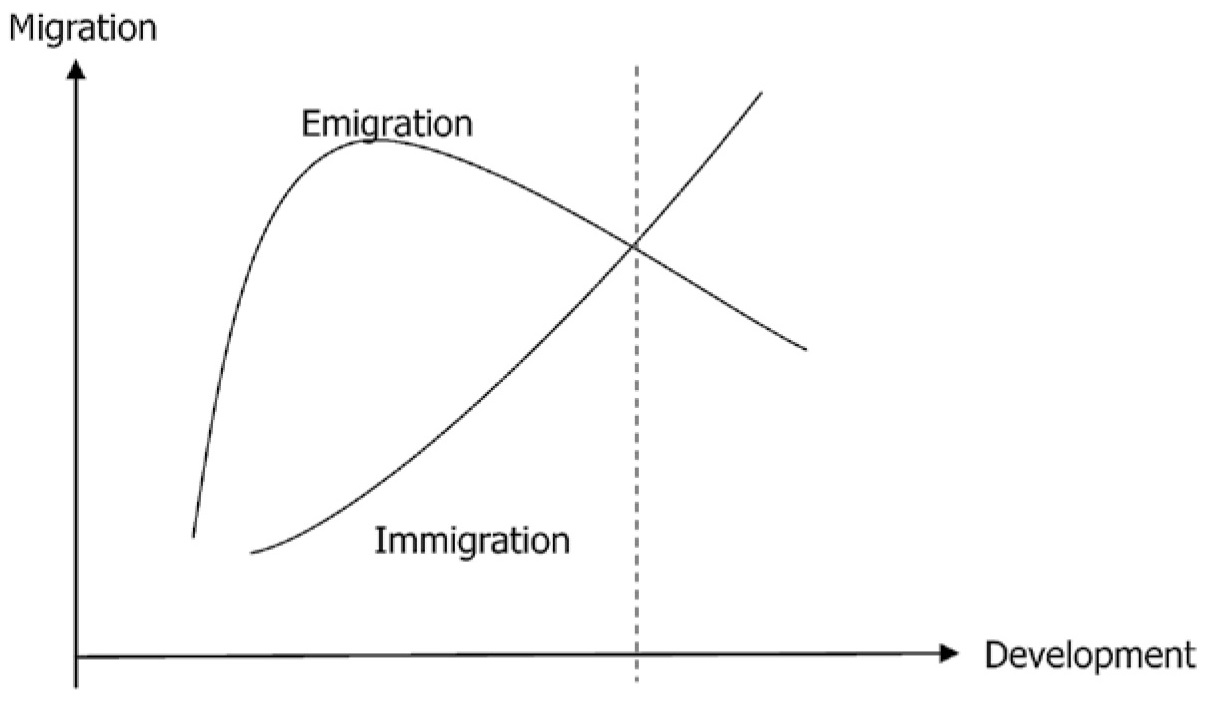
\includegraphics{./tex2pdf.-8c1f0593c1a83dbe/b95ff94df58c181782faebced34fbdcebfed67d6.jpg}
\caption{Transición migratoria (de Haas et~al.,
2015).}\label{fig:trans_migra}
}
\end{figure}

Las críticas a esta teoría se asemejan a algunas de las vertidas con
respecto a la transición demográfica propiamente dicha. Según Skeldon
(2012): es esencialmente una descripción a nivel macro basada en la
experiencia de Europa occidental y Norteamérica, que relaciona en forma
intuitiva los cambios hipotéticos en las migraciones con los cambios en
fecundidad y mortalidad (traducción propia).

\hypertarget{diuxe1logo-entre-migraciones-internacionales-e-internas}{%
\subsubsection{Diálogo entre migraciones internacionales e
internas}\label{diuxe1logo-entre-migraciones-internacionales-e-internas}}

Los procesos migratorios son la suma de un complejo conjunto de factores
e interacciones que llevan a individuos y familias a migrar, y que luego
influencian en el curso de dicha migración.

¿Cómo se pueden relacionar las teorías de la migración internacional con
los abordajes de migración interna?. King y Skeldon (2010) proponen
algunos puntos de contacto a partir de los cuales se pueden establecer
vínculos entre ambos marcos teóricos, aunque en primer lugar traen a
discusión la diferenciación entre dichos tipos de migración, ya que a
veces el límite entre ellas puede ser difuso, dado que la distancia
puede no tener una relevancia central (ej.: una migración interna de
miles de kilómetros dentro de un país grande, como EE.UU., Rusia, China
o Brasil, en comparación con una entre estados fronterizos europeos). A
su vez existen nuevos ``tipos'' de fronteras, como el espacio Schengen
en Europa, y las fronteras pueden cambiar de acuerdo a los vaivenes
(geo)políticos. De todas formas los autores reconocen la división entre
ambas migraciones, entendiendo que sí hay una diferencia entre el
individuo que migra dentro de su estado y el que lo hace hacia otro.

Los autores proponen el esquema de la~fig.~\ref{fig:migration_pathways}
para graficar las posibles continuidades o ``escalonamientos'' entre
ambos tipos de migraciones, identificando 10 caminos posibles para la
migración en función de su carácter de interna o internacional y de la
posibilidad del retorno:

\begin{figure}
\hypertarget{fig:migration_pathways}{%
\centering
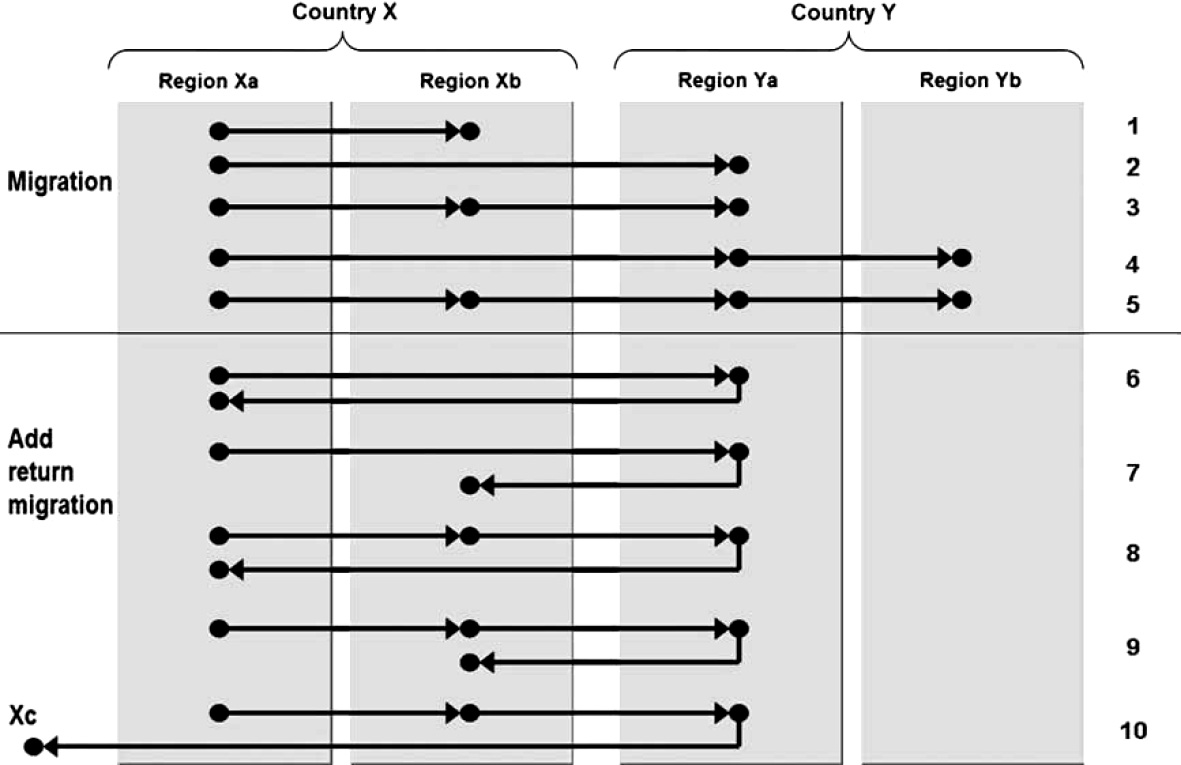
\includegraphics{./tex2pdf.-8c1f0593c1a83dbe/a6bbc6a663a610e2b1631c3e3acad8b417f7424a.jpg}
\caption{Los 10 caminos de las migraciones (``migration pathways'')
identificados por King y Skeldon (2010).}\label{fig:migration_pathways}
}
\end{figure}

Según el esquema, \emph{X} e \emph{Y} representan a dos países
diferentes. A su vez, \emph{Xa}, \emph{Xb}, \emph{Ya} e \emph{Yb} son
regiones dentro de esos países ficticios, donde \emph{Xa} es una región
rural, \emph{Xb} es un centro urbano (como una ciudad capital),
\emph{Ya} es una ciudad principal e \emph{Yb} una región provincial.

Con respecto a la integración teórica, las hipótesis de la transición de
la movilidad de Zelinsky (1971), ya mencionadas anteriormente, son
consideradas el intento más ambicioso en ese sentido (King y Skeldon,
2010). Para Zelinsky existía una aumento en las movilidades en el
espacio-tiempo y esta regularidad era un componente del proceso de
modernización (Skeldon, 2012).

Las críticas a dicho vinculo son las siguientes:

\begin{itemize}
\item
  Presentan una visión idealizada de las sociedades pre-modernas,
  concibiéndolas como sociedades estáticas en las cuales los movimientos
  de población eran muy poco comunes.
\item
  El paralelismo y continuidad entre la transición demográfica y la
  migratoria sin aportar evidencia de cómo se influenciaban mutuamente.
\item
  El anclaje en una visión anticuada de modernidad y desarrollo, el
  progresismo teleológico con ``occidente'' como espejo.
\end{itemize}

Los aportes de Pryor (1981) también se orientan a la integración de
ambas vertientes, aunque el resultado es una propuesta para la
integración teórica, sin llegar a ninguna demostración empírica de como
realizar dicha integración. King y Skeldon (2010) presentan tres
aproximaciones en las que se puede lograr cierto grado de ``fusión''
entre las teorías de migración interna e internacional: el análisis de
sistemas, la integración de migrantes y la migración y el desarrollo.

Con respecto a la teoría de sistemas, se destaca la inexistencia de
estudios empíricos basados en ella, que atribuyen a la ausencia de datos
que permitieran operacionalizarla. Ese problema se agrava si se tiene en
cuenta la ausencia de consenso académico en torno a lo que es un
``sistema migratorio''. Sin embargo, existen abordajes que han utilizado
los sistemas migratorios para el estudio de migraciones internacionales
(King y Skeldon, 2010). Finalmente, se valora la potencia de la
integración de varios tipos de migraciones, así como disciplinas y
paradigmas, en tanto es una teoría flexible, que puede ser vinculada a
un abordaje basado en la economía política, si en el sistema se
demuestra la importancia de los vínculos pasados entre origen y destino,
ya sea por la colonización, influencia política, comercio, inversiones o
lazos culturales (King y Skeldon, 2010).

En segundo lugar, se refiere a los procesos de integración o
incorporación de migrantes. Es claro que los migrantes internos también
viven procesos e incorporación, basta imaginar contextos de migración
rural-urbano y las diferencias que implican ambos medios (Elizaga y
Macisco, 1975). Los autores presentan la definición de integración que
consideran convencional (``mainstream''), vertida por Heckmann (2005):
integración como la aceptación de los migrantes en las instituciones más
importantes, las relaciones y estatus de la sociedad receptora, en tanto
que para los migrantes refiere al proceso de aprender una nueva cultura,
adquirir derechos, acceder a posiciones y estatus, construir relaciones
personales con personas de la sociedad receptora y desarrollar
sentimientos de identificación con la misma. Posteriormente ponen a
discusión esa definición con otras, en tanto la sociedad receptora no es
monolítica y la integración puede significar cosas diferentes para
personas o colectivos. Consideran que en esas diferentes ``esferas de la
integración'' es que se puede trazar un paralelo entre las dimensiones
interna e internacional.

El tercer aspecto es relativo al desarrollo como integrador teorías
migratorias. Ha habido investigaciones sobre los nexos entre la
migración internacional y la promoción del desarrollo, por ejemplo en lo
relativo a las remesas o a las políticas de retorno. Sin embargo sobre
migraciones internas no ha habido abordajes que atiendan esos nexos,
aunque la importancia de dichas migraciones sean mayor que la
internacional en algunos países, por ejemplo en China (King y Skeldon,
2010).

A modo de cierre, vale citar a Massey et. al. (2000), quienes hace casi
30 años afirmaban algo que consideramos aún vigente: ``En el presente no
hay una teoría coherente y única sobre la migración internacional,
solamente un conjunto fragmentado de teorías que se han desarrollado en
buena medida aisladas unas de otras, algunas veces pero no siempre
segmentadas por las fronteras disciplinarias'' (p.~6). De todas formas
se coincide con King y Skeldon (2010) en qué, a pesar de la necesidad de
teorizar y construir vínculos entre las teorías, el intento de
construcción de una teoría que abarque todos los tipos de migraciones,
en todos los períodos de tiempo y espacios geográficos permanece como un
fin ilusorio y reduccionista.

\hypertarget{el-espacio-geogruxe1fico-en-las-migraciones}{%
\subsection{El espacio geográfico en las
migraciones}\label{el-espacio-geogruxe1fico-en-las-migraciones}}

Siendo un concepto clave en el pensamiento geográfico, la definición de
espacio es de gran complejidad. Históricamente el concepto de espacio
viene ligado al interés de mapear objetos, lugares, fenómenos y
personas, intrínsecamente relacionado con el ejercicio del poder, y
facilitado por determinadas tecnologías (Gregory et~al., 2009).

Se puede identificar un primer abordaje en geógrafos como Humboldt y
Hettner primero, seguidos por Hartshorne, quién toma la teoría de los
geógrafos alemanes del siglo XIX mencionados con antelación, y tienen
como con antecedentes a Kant, Newton y Descartes. Este abordaje implica
la concepción del espacio como algo ``absoluto'', es decir algo
universal y concebible como fuera de existencia humana (Harvey, 2007;
Hubbard y Kitchin, 2010), una ``caja'' en la cual las cosas existen y
los eventos tiene lugar (Gregory et~al., 2009), o como mero
``contenedor'' (López Trigal et~al., 2015), dentro del cual el mundo
acontece (Clifford, 2009). Ese espacio absoluto donde los eventos están
fijados sería el objeto de la Geografía, por otro lado el tiempo sería
el objeto de la Historia (Harvey, 2007). A su vez, Hartshorne consideró
a la Geografía como una ciencia ideográfica\footnote{La distinción entre
  ciencias nomotéticas e ideográficas proviene del filósofo alemán W.
  Windelband. Las ciencias nomotéticas son aquellas que buscan
  generalidades, coincidentes con las denominadas ciencias naturales o
  exactas, en tanto las ciencias ideográficas estudian los fenómenos
  particulares e individuales, con características irrepetibles, y
  coinciden con las disciplinas sociales e históricas (Solís, 2005).} es
decir que se ocupaba del análisis de eventos particulares con
características únicas (Gregory et~al., 2009).

La noción decimonónica de espacio-contenedor no representa un marco
adecuado para la presente investigación, dado que se entiende que el
espacio cumple un rol en la conformación de los fenómenos a estudiar.
Considerar al espacio como mero contenedor de la sociedad sería
desconocer el papel de la sociedad en la construcción del espacio y el
rol del espacio en la conformación de las sociedades. Atendiendo a las
migraciones en particular, parece aún menos plausible que los flujos
migratorios se den en un espacio-contenedor y que la ocurrencia de
dichos flujos no tenga una influencia en dicho espacio, como ejemplo
vale mencionar los cambios en los estados nacionales derivados de la
ocurrencia de migración, cambios que en algunos casos son fundacionales,
como ser en aquellos países con pasado colonial. Sin embargo vale
mencionar que el espacio absoluto es, en general, el abordaje implícito
en los Sistemas de Información Geográfica, o en sentido más amplio y
usando el término en inglés, en la ``Geographical Information Science''
(Kitchin y Thrift, 2009).

Hacia mediados del siglo XX comienzan a surgir nuevas
conceptualizaciones del espacio, entre ellas la propuesta por Fred K.
Schaefer, como crítica al pensamiento de Hartshorne. Schaefer sostuvo
que las relaciones eran entre objetos y eventos, no entre un sistema de
coordenadas fijo y externo, por ende el espacio era relativo a los
eventos y objetos que constituyen un sistema espacial o una estructura
espacial. Estamos ante la emergencia de la \textbf{concepción
relativista de espacio}, que tuvo en Albert Einstein su antecedente
(Harvey, 2007). A su vez, Schaefer atacó la idea del
\textbf{``excepcionalismo''} geográfico, homologando la Geografía a
otras ciencias, con metodologías compartidas y con el objetivo de
estudiar las relaciones espaciales para identificar leyes universales;
atribuyó la incapacidad de detectar leyes en el pensamiento de
Hartshorne a la concepción ideográfica de la Geografía, reducida a la
descripción e identificación de regiones (Gregory et~al., 2009; Warf,
2006). Entre esas leyes, por ejemplo, se encontraría la del decaimiento
con la distancia o \emph{distance decay} (Kuhlke, 2006), que será
analizada en el presente trabajo, dentro del apartado dedicado a la
interacción espacial. El espacio relativo tuvo al análisis espacial como
su técnica predilecta, lo cual implicaba la abstracción del espacio
físico para convertirlo en un espacio matemático (Gregory et~al., 2009).

Durante los años 50s y 60s, tomando la iniciativa de Schaefer, geógrafos
de la Universidad de Washington en Seattle (Estados Unidos), comenzaron
lo que hoy conocemos como la \textbf{``revolución cuantitativa''}
(Kuhlke, 2006). Su objetivo fue transformar a la Geografía en una
ciencia espacial positivista, buscando la formulación de leyes
espaciales, basándose en el análisis estadístico (Hubbard y Kitchin,
2010). La geografía cuantitativa, en ocasiones llamada geografía
teorética, empleó técnicas estadísticas, geometría (por ejemplo en la
teoría de grafos) y analogías con las ciencias naturales (Corrêa, 1990).
Según la visión de sus protagonistas estos cambios tenderían a
consolidar a la Geografía como una ciencia espacial formal, una ``nueva
geografía'' orientada a la búsqueda de un ``orden espacial''
preexistente, evidenciable mediante las herramientas y métodos de esta
novel disciplina (Gregory et~al., 2009). La pretensión de búsqueda de
leyes, es decir las intenciones de encontrar generalidades, sustentan el
nombre de geografía teorética.

El auge de la geografía cuantitativa pavimentó el camino para el
surgimiento de los abordajes basados en modelos espaciales predictivos,
entre ellos los modelos de interacción espacial, siendo Allan Wilson uno
de sus principales referentes (1971).

Hacia la década de los 70s, alentados por los cambios políticos,
económicos y culturales que estaban teniendo lugar, el abordaje
cuantitativo comienza a ser duramente cuestionado, calificado de
positivista, carente de sustentos teóricos y de potencia explicativa, al
tiempo que surgen nuevos abordajes cualitativos (Birkin y Clarke, 2019):
estamos ante el nacimiento de la geografía crítica (Corrêa, 1990).

Los críticos identificaron un ``fetichismo espacial'' en la geografía
cuantitativa, dado que las relaciones sociales pretendían ser tratadas
puramente como relaciones espaciales. Esta crítica dio lugar a nuevos
abordajes orientados al análisis de procesos, introduciéndose el
concepto de ``espacio relacional'', según el cual el espacio está
imbricado en las relaciones sociales a través de las prácticas (Gregory
et~al., 2009). Desde la perspectiva del espacio relacional, se entiende
que el espacio absoluto y relativo no se pueden separar, y torna la
mirada hacia los sistemas sociales que producen diferentes estructuras
espaciales (Kuhlke, 2006). En ese sentido, el espacio es un agente
(entre otros) en la construcción de las relaciones sociales y
económicas, y a su vez es construido por dichas relaciones y prácticas
sociales (Kitchin y Thrift, 2009). Esta visión fue introducida
primeramente por los denominadas geógrafos radicales, por ejemplo los
marxistas o feministas (Kitchin y Thrift, 2009).

Posteriormente, entrada la década de los años 80s, los abordajes
cuantitativos y la modelación espacial volvieron a cobrar relevancia,
facilitadas por las nuevas posibilidades brindadas por los avances en
tecnologías informáticas, y en particular por la mayor capacidad de
cómputo (Birkin y Clarke, 2019).

En los párrafos anteriores se intentó resumir en forma muy somera el
devenir teórico de la Geografía, en particular en su relación con el
concepto de ``espacio'', cuya definición es siempre elusiva y responde a
la concepción teórica desde la cual se lo aborda. En suma, se
identificaron tres grandes acepciones del espacio: absoluto, relativo y
relacional.

En cuanto a la complejidad del fenómeno y su relación con las diferentes
acepciones del espacio geográfico, vale mencionar las diferentes
conceptualizaciones que se pueden hacer de la ``distancia'', enunciadas
por Waldo Tobler (2004): métrica, elipsoidal, en unidades de tiempo o
costo de viaje, distancia Manhattan, riemmanianas o de Finsler,
distancia social, topológica y ordinal; a las que cabría agregar la
distancia funcional (Claeson, 1968). Todas estas concepciones de
distancia se relacionan con un abordaje diferente del espacio
geográfico, y como consecuencia ``proximidad'' o ``lejanía'' pueden
significar cosas diferentes según cada concepción (Tobler, 2004). A modo
de ejemplo, señalamos otro aspecto de gran relevancia: la percepción de
la distancia, la cual es necesariamente subjetiva y su importancia no es
menor en tanto que los movimientos migratorios tienen por protagonistas
a sujetos (Claeson, 1968), Esto refiere a que el espacio vivido difiere
plenamente de aquel espacio absoluto, en tanto los comportamientos
espaciales humanos están basados un espacio cognitivo, es decir una
construcción del pensamiento (Kitchin y Thrift, 2009). Sin embargo, la
posibilidad de operacionalizar la percepción espacial, en este caso la
de las distancias, implicaría un trabajo cualitativo y escapa a los
objetivos de la presente investigación.

Esta visión del espacio cognitivo se asocia a corrientes contemporáneas
relacionadas con el existencialismo y fenomenología (abordajes
ontológicos). Otras se basan en el marxismo crítico o son de raíz
post-estructuralista, abrevando en el pensamiento de Foucault, Deleuze y
Lacan. Siguiendo las teorizaciones compartidas por los abordajes
contemporáneos planteadas por Gregory (2009), el fenómeno de la
migración y el marco teórico que se propone en la presente investigación
se pueden relacionar con la idea del espacio y el tiempo como entidades
integradas, generando un campo móvil, descartando la noción del espacio
como algo fijo y del tiempo como exclusivamente dinámico. Habiendo
descartado el ``espacio absoluto'' como posibilidad, queda por responder
la siguiente pregunta: ¿qué concepto de espacio se considera más afín al
abordaje de las migraciones que sea realizará en este trabajo?. Para dar
respuesta será de utilidad la categorización realizada por Nigel Thrift
(2008): la construcción empírica del espacio, el espacio de la imagen,
el espacio del lugar y el espacio de flujos.

Por \textbf{``construcción empírica del espacio''} se refiere a aquellas
cosas que mantienen nuestro espacio, ese tejido de la vida cotidiana, en
funcionamiento: los sistemas de medidas, la estandarización del tiempo,
las formas cada vez más exactas de registrar el espacio físico (GPS,
SIGs) y la creciente estandarización del espacio permitida por ésas
tecnologías.

El \textbf{espacio de la imagen} refiere a la emergencia de la imagen
como forma en la cual registramos el espacio que nos rodea y sus
posibles cambios futuros. A su vez, su proliferación ha cambiado la
forma en como aprehendemos el espacio.

El \textbf{espacio del lugar} refiere a aquella concepción en la cual el
espacio es concebido como un lugar. Los lugares son más cercanos a la
experiencia humana que el concepto más abstracto de espacio; en los
lugares los cuerpos pueden vivir (al menos aproximadamente) la idea
occidental de lo que debería ser ``ser humano''. Refiere al espacio
naturalizado en nuestra vida cotidiana.

El \textbf{espacio de los flujos} refiere a las conexiones que sustentan
la interacción de eso que conocemos como ``mundo''. Refiere a todo tipo
de flujos, movimientos cotidianos de trabajadores, turistas, flujos
comerciales, los de información a través de la televisión, radio o
internet, o los flujos de dinero (electrónicos o físicos). Dichos flujos
cobran cada vez relevancia en tanto la ``globalización'' se profundiza.
Al estar cada vez más interconectados, el concepto de ``escala'' permite
detenerse sobre particularidades que quieran ser estudiadas o abarcar la
globalidad si ese es el objetivo.

Entonces, como se podrá intuir, nos hemos acercado a una concepción del
espacio más afín al abordaje del presente trabajo, entiendo las
migraciones como parte de ese espacio de flujos. Los otros tipos de
espacio también se pueden relacionar con en el fenómeno de las
migraciones, a modo de ejemplo pensemos en el espacio de las imágenes
sobre lugar de destino y de origen que conforman los imaginarios de las
personas que migran, o en el sentido de lugar a partir del cual las
poblaciones migrantes generan lazos con determinados espacios en su país
o región de destino, produciendo ``lugares'', constituyéndose
posiblemente como los primeros pasos en un proceso de asimilación. Sin
embargo estos abordajes se consideran más atinados para un enfoque
cualitativo y no serán centrales a este trabajo.

El espacio de flujos conformado por y en torno a las migraciones es
destacable. La migración en sí, el movimiento de una o varias personas
(juntos con determinada cantidad de bienes personales y/o capital) para
asentarse por un período de tiempo considerable en un destino
determinado, puede ser vista como un flujo. A su vez, ese flujo puede
desencadenar otros entre el origen y el destino de la migración: flujos
de información, de transporte, de capital, culturales, de nuevos
migrantes, de retorno, entre otros.

Cambiando la escala de análisis, es posible relacionar el espacio de
flujos con otros fenómenos que trascienden las dinámicas internas. Por
ejemplo, la oferta de puestos de trabajo en determinada localidad puede
ser un gran atractor, y generar migraciones de mano de obra desde una o
varias localidades cercanas. A su vez, este proceso puede estar
insertado en flujos globales, como los flujos de capital o la
consolidación nuevas filiales industriales por parte de empresas
multinacionales (Trajtenberg, 1999). Por otro lado, la provisión de
personal técnico o profesional altamente calificado y los cargos de
gerencia pueden implicar migraciones desde otros países, facilitados por
la propia empresa, siendo el país de origen de la multinacional uno de
los posibles orígenes.

Además de las concepciones de espacio vertidas, los aportes de geógrafos
latinoamericanos también pueden brindar herramientas útiles para
conceptualizar el espacio. El geógrafo brasileño Roberto Lobato Corrêa
(1990), en un abordaje basado en Marx y Lefebre, considera a la
Geografía como una ciencia social, por ende su objeto de estudio es la
sociedad, aunque se objetiva de forma diferente que en otras ciencias
sociales. La objetivación de la Geografía la orienta al \textbf{estudio
de la organización espacial}. Dicha organización espacial tiene su
materialidad, es una ``segunda naturaleza'', originada en la
transformación de la naturaleza primitiva mediada por las relaciones
sociales de producción, una naturaleza ``antropizada''. Si pensamos en
la migración interna, ciertos aspectos de esa materialización están
presentes en las configuraciones de los patrones migratorios. Las
\textbf{``rugosidades''} (expresión que Corrêa toma de Milton Santos),
en tanto marcas del pasado fijadas en el espacio, permanecen y se
evidencian, por ejemplo, cuando determinada ciudad concentra gran parte
de las funciones, la población y las actividades económicas. Dicha
urbanización seguramente funcione como un atractor de población, en
tanto haya gran oferta de servicios y oportunidades económicas, entonces
la organización espacial también está ejerciendo una influencia en la
configuración de determinados movimientos migratorios.

Descartando la posibilidad de un espacio absoluto, se considera que
ciertas características de ese espacio de flujos se pueden modelar,
aceptando que todo modelo es un simplificación y que sería reduccionista
pensar que algo tan complejo como el espacio, la sociedad y los sujetos
puede explicarse del mismo modo.

\hypertarget{la-interacciuxf3n-espacial-y-su-modelaciuxf3n}{%
\subsection{La interacción espacial y su
modelación}\label{la-interacciuxf3n-espacial-y-su-modelaciuxf3n}}

La expresión ``interacción espacial'' fue popularizada por el geógrafo
estadounidense Edward Ullman en 1954, para indicar la interdependencia
entre regiones geográficas (de Castro Catão et~al., 2010; Gregory
et~al., 2009). Refiere a cualquier movimiento de personas, información o
bienes en el espacio, resultante de un proceso de toma de decisiones
(Fotheringham, 2001). Por ejemplo: las decisiones asociadas un flujo
comercial, que implican vender determinada mercadería y transportarla
hacia el destino donde reside el comprador, generando un flujo de
capital inverso, es decir del comprador al vendedor. Otro ejemplo
podrían ser los flujos de personas de localidades diversas a un sitio
concreto, que puede estar ligadas a un determinado atractivo, como ser
el acceso a determinados servicios (educación, salud, espectáculos). A
su vez se destaca la noción de interdependencia entre los lugares, dado
que un flujo, por ejemplo un flujo migratorio, puede dar inicio otros
flujos nuevos, por ejemplo flujos comerciales, culturales, de capital,
de información, de pasajeros, entre otros. Es así que las interacciones
espaciales pueden variar en el espacio y en el tiempo, presentando
patrones espaciales que se articulan y complementan (de Castro Catão
et~al., 2010). Se constata un aumento de la magnitud y la complejidad de
los flujos en general, debido al desarrollo de la economía capitalista y
su globalización, favorecida por los avances científicos y técnicos que
posibilitan la ``superación del espacio por el tiempo'' (de Castro Catão
et~al., 2010). Según David Harvey, basándose en Marx, el capitalismo
encoje las distancias creando una compresión espacio-temporal en sus
esfuerzos para desterritorializarse y reducir la ``fricción'' de la
distancia (Gregory et~al., 2009; Harvey, 2007). A su vez, el accionar
capitalista crea nuevas relaciones espaciales, principalmente mediante
la inversión en transporte y comunicaciones (Harvey, 2007); como
ejemplos basta pensar en las redes de carreteras y vías férreas, o en el
desarrollo de internet.

Las interacciones espaciales reflejan la desigualdad entre lugares y se
caracterizan por la asimetría, favoreciendo un lugar determinado en vez
de otro, ampliando las desigualdades previamente existentes. Es a través
de las redes que estas interacciones espaciales se realizan, por ejemplo
las redes de transporte que permiten el flujo de personas o bienes de un
lugar a otro (de Castro Catão et~al., 2010). La noción de las
interacciones espaciales como reflejos de la desigualdad en el espacio
tiene en los procesos migratorios un claro ejemplo. Si consideramos al
flujo de migrantes como una interacción espacial (y así lo haremos en la
presente investigación) podemos aventurar algunas hipótesis, por
ejemplo, que las personas que migran lo hacen hacia destinos donde se
concentran servicios y oportunidades económicas, en particular
oportunidades de empleo. Sería contraintuitivo que los migrantes elijan
aquellas localidades más aisladas, con menos conexiones, con escasez de
servicios, con economías pequeñas y poco dinámicas. Entonces, los flujos
migratorios tenderán a ser hacia aquellos lugares que presenten los
atractores mencionados, por ejemplo las grandes ciudades o las
localidades con mayor dinamismo económico y buena provisión de
servicios, reforzando una desigualdad territorial previamente existente.
En el mismo sentido, las migraciones internacionales tienen a dirigirse
desde los países insertos de forma subalterna en la economía global
(aunque no necesariamente de los países menos desarrollados) hacia a
aquellos países más desarrollados.

Las interacciones espaciales y los flujos que las integran son pasibles
de una descripción matemática: los modelos de interacción espacial.
Estos modelos sirven a dos propósitos generales, la predicción de flujos
desconocidos y la obtención de información sobre los determinantes del
sistema de flujos que se analiza (Fotheringham, 2001). Los modelos de
interacción espacial son una de las técnicas más usadas para entender
los flujos de personas y bienes entre localidades, enfatizando en la
importancia que tiene el ``lugar'' en el proceso de modelación (Gulden
et~al., 2019).

Los flujos de población se pueden conceptualizar como intercambios entre
dos entidades, los orígenes y los destinos, que tienen diferentes
propiedades de emisividad y atracción (Dennett, 2018). La fuerza de
dicha interacción radica en las propiedades de los orígenes y destinos y
en la influencia negativa del costo, el cual usualmente se presenta
asociado a la distancia (\emph{distance decay}). Esto quiere decir que
costos altos debilitarán o desestimularán los flujos, en tanto que
costos bajos los fortalecerán o estimularán. Si el factor de costo es la
distancia, dicho costo aumentará en tanto los orígenes y destinos estén
más lejos en el espacio y viceversa. El ``decaimiento con la distancia''
refiere a la atenuación de un patrón con la distancia, en relación con
un punto central (Gregory et~al., 2009). La importancia de este concepto
está vinculada a la denominada ``primera ley de la geografía'' de Waldo
Tobler: ``todo está relacionado con todo, pero aquello más cercano entre
sí está más relacionado que aquello lejano'' (Tobler, 1970).

Las definiciones de atracción o ``masa'' entendidas como las
características atractoras o expulsoras por un lado, y la ``fuerza''
entendida como los flujos entre dos entidades por otro, son una analogía
con ley de gravedad de Newton, lo cual determinó que su denominación
inicial fuera ``modelos gravitacionales'' (Delgado, 2003; Molho, 1986).

Es posible interpretar la relación entre localidades y departamentos
como una red o grafo, donde cada nodo es origen/destino, la conexión
entre ellos, denominada ``arco'', es el flujo de personas y el ``peso''
de esa conexión es la magnitud de ese flujo. Sobre dicho ``peso'' se
pueden aplicar ponderadores como la distancia/costo (Miranda, 2012). En
una red de n localidades, existen (n x n ) -- n arcos direccionales
posibles, si se excluyen las conexiones de un nodo consigo mismo (Chun,
2008). La red puede ser física, por ejemplo la red de transporte, o
abstracta. Para el caso del análisis de las migraciones, si tomamos en
cuenta que lo que interesaría es la magnitud de personas que migran y
nos los caminos que usan para migrar, la red sería abstracta (Chun,
2008). Vale mencionar que la referencia a redes no refiere a la teoría
de ``redes migratorias'' (de Haas et~al., 2015).

El término ``distancia'' en general refiere a la distancia física en
este abordaje, pero sabemos que las percepciones subjetivas de la
distancia varían de persona a persona y dicha subjetividad podría ser
relevante en un fenómeno que tiene un componente relativo a una decisión
humana (Claeson, 1968). Entre los primeros antecedentes de los modelos
de interacción espacial se encuentran los aportes de Reilly (Reilly,
1931), quien analizando actividades comerciales propuso una relación
positiva entre la magnitud de flujos de consumidores entre localidades y
la población residente en dichas localidades, en tanto que una relación
negativa con el cuadrado de las distancias que las separa (Garrocho,
2003). Reilly se basó en esos dos supuestos para elaborar un sencillo
modelo, a posteriori denominado ``Ley de Reilly'' y que fue simiente de
los futuros modelos de interacción espacial.

Más cerca en el tiempo, los aportes de Allan Wilson (1971) complejizan
los primigenios abordajes ``gravitacionales''. Wilson introduce el
concepto de ``modelos de interacción espacial'', dejando atrás la
nomenclatura de inspiración newtoniana. Además, propone una mejor
justificación teórica, proponiendo una familia de cuatro modelos,
diferenciados por la información conocida para limitar o condicionar los
valores que la interacción puede tomar. En su esencia, los modelos de
interacción espacial son formas estadísticas del modelo gravitatorio,
incluyendo como factores la población en origen y en destino, la
distancia entre ellos y alguna medida de competencia o atractividad
(Raymer, 2007).

Teniendo los aportes de Wilson como basamento, los modelos de
interacción espacial han sido aplicados a fenómenos de diversa índole,
como migraciones, transporte público y movilidades pendulares, análisis
locacional (orientado a la localización de actividades comerciales, por
ejemplo), entre otros tópicos (Fotheringham, 2001; Mallozzi, 2017). Esa
variedad de aplicaciones se puede asociar a la capacidad explicativa y
predictiva de los modelos (Santos, 1994).

\hypertarget{antecedentes-del-estudio-de-la-migraciuxf3n-interna-en-uruguay}{%
\subsection{Antecedentes del estudio de la migración interna en
Uruguay}\label{antecedentes-del-estudio-de-la-migraciuxf3n-interna-en-uruguay}}

Los primeros antecedentes se centraron en la exploración de las causas
de la migración rural-urbana y el consecuente declive de la cantidad de
personas viviendo en zonas rurales (Macadar y Domínguez, 2008),
estableciendo una asociación entre la producción agrícola intensiva, las
urbanizaciones intermedias y el mayor desarrollo de la región sur, y por
otro lado las prácticas extensivas y el desarrollo de ``ciudades
primadas'', es decir ciudades concentradoras de población y recursos
económicos por oposición a un medio rural poco poblado y poco dinámico
económicamente (Macadar y Domínguez, 2008).

Las principales fuentes cuantitativas para el estudio de la migración
interna en Uruguay son los censos de población, que en la segunda mitad
del siglo XX fueron ejecutados en 1963, 1975, 1985, 1996 y 2011.

En línea generales, Montevideo presenta una tendencia al estancamiento
en el crecimiento de su población desde el año 1963 (Bengochea, 2011) y
una pérdida de población desde el 1996, debido a la radicación de
personas en Canelones y San José, particularmente Ciudad de la Costa así
como la emigración internacional, dado que gran parte de los emigrantes
internacionales residían en Montevideo (Bengochea, 2011; Koolhaas,
2013).

A partir de los datos del Censo de 1985 se constata una
\textbf{reducción del atractivo de la zona litoral, suroeste y de
Montevideo}, creciendo las localidades que conforman el área
metropolitana de la capital (Macadar y Domínguez, 2008), al tiempo que
adquiere importancia como región receptora el noroeste del país,
asociada al tipo de cambio favorable y las dinámicas de la frontera con
Brasil (Bengochea, 2011; Macadar, 1995). No obstante lo mencionado, las
principales corrientes migratorias siguieron teniendo como origen y
destino al departamento de Montevideo (Calvo, 1995).

El censo de 1996 permite identificar un aumento importante de la
población en la costa del departamento de Canelones junto con el ya
mencionado decrecimiento poblacional en Montevideo (Bengochea, 2011;
Pellegrino, 2009). A su vez se identifica un saldo migratorio negativo
de los departamentos de la frontera noreste para con Montevideo,
revirtiéndose el fenómeno que aconteció durante la década de los 80s
(Macadar y Domínguez, 2008) y emerge el departamento de Maldonado como
atractor de migración interna (Bengochea, 2011).

Según los datos del Censo INE 2011, solamente los departamentos de
Maldonado, Canelones, San José, Colonia, Salto y Río Negro ha habido un
aumento de la población (Koolhaas, 2013). A su vez, dentro de esos
departamentos, solo Maldonado, Canelones, San José, Colonia y Salto
tuvieron un saldo migratorio interno positivo (Koolhaas, 2013). En
particular Canelones y Maldonado, ambos departamentos costeros,
presentan crecimiento poblacional desde el censo de 1963 (Bengochea,
2011; Koolhaas, 2013), en parte asociado a la expansión de la ciudad de
Montevideo (procesos de suburbanización), la generación de nuevas
centralidades y el crecimiento de Maldonado (y su propio proceso de
suburbanización).

\hypertarget{tbl:mig_recientes}{}
\begin{longtable}[]{@{}lllllllll@{}}
\caption{\label{tbl:mig_recientes}Migrantes recientes según los censos
1975, 1985 y 1996 (Bengochea, 2011; Macadar y Domínguez, 2008) y 2011
(elaboración propia con datos del INE (2011c)).}\tabularnewline
\toprule
cat. & 1970/1975 & \% & 1980/1985 & \% & 1991/1996 & \% & 2006/2011 &
\%\tabularnewline
\midrule
\endfirsthead
\toprule
cat. & 1970/1975 & \% & 1980/1985 & \% & 1991/1996 & \% & 2006/2011 &
\%\tabularnewline
\midrule
\endhead
Migrante & 160.341 & 5,8\% & 181.541 & 6,1\% & 180.404 & 5,7\% & 148.759
& 4,5\%\tabularnewline
No migrante & 2.628.088 & 94,2\% & 2.773.700 & 93,9\% & 2.983.359 &
94,3\% & 3.137.118 & 95,5\%\tabularnewline
Total & 2.788.429 & 100\% & 2.955.241 & 100\% & 3.163.763 & 100\% &
3.285.877 & 100\%\tabularnewline
\bottomrule
\end{longtable}

La migración es más intensa en las edades económicamente activas y en
los jóvenes (Koolhaas, 2013). La migración reciente tiene más incidencia
en mujeres jóvenes, probablemente asociada a la feminización de la
matrícula universitaria y a la atracción de Montevideo por la existencia
de mayor oferta laboral para las mujeres (Bengochea, 2011).

La propensión a migrar de los jóvenes se puede comprender atendiendo a
las características de ese período vital: formación de pareja, inicio de
la vida reproductiva, inicio de estudios terciarios, inicio de la vida
laboral, etc. (Koolhaas, 2013).

También se ha identificados el perfil más joven y feminizado de quienes
migran hacia Montevideo. Por otro lado, el perfil de familias completas
de quienes migran desde Montevideo, integradas por parejas de entre 30 y
40 años con niños, probablemente debido a un ciclo de expansión de
dichas familias (Bengochea, 2011).

\newpage

\hypertarget{marco-metodoluxf3gico}{%
\section{Marco metodológico}\label{marco-metodoluxf3gico}}

\hypertarget{fuentes-de-informaciuxf3n}{%
\subsection{Fuentes de información}\label{fuentes-de-informaciuxf3n}}

La principal fuente de información para el presente trabajo serán los
censos 1996 y 2011 realizados por el Instituto Nacional de Estadística
(INE). En particular los censos 1996 y 2011 incorporaron preguntas
relativas a la migración interna y se presentan en el siguiente cuadro.

\begin{longtable}[]{@{}ll@{}}
\caption{Preguntas relevantes para el análisis de la migración interna
en los censo INE 1996 y 2011.}\tabularnewline
\toprule
\begin{minipage}[b]{0.47\columnwidth}\raggedright
Preguntas en censo 1996\strut
\end{minipage} & \begin{minipage}[b]{0.47\columnwidth}\raggedright
Preguntas en censo 2011\strut
\end{minipage}\tabularnewline
\midrule
\endfirsthead
\toprule
\begin{minipage}[b]{0.47\columnwidth}\raggedright
Preguntas en censo 1996\strut
\end{minipage} & \begin{minipage}[b]{0.47\columnwidth}\raggedright
Preguntas en censo 2011\strut
\end{minipage}\tabularnewline
\midrule
\endhead
\begin{minipage}[t]{0.47\columnwidth}\raggedright
En qué localidad o paraje vive habitualmente\strut
\end{minipage} & \begin{minipage}[t]{0.47\columnwidth}\raggedright
Localización de la vivienda/hogar/persona\strut
\end{minipage}\tabularnewline
\begin{minipage}[t]{0.47\columnwidth}\raggedright
En qué localidad o paraje paso a vivir cuando nació\strut
\end{minipage} & \begin{minipage}[t]{0.47\columnwidth}\raggedright
Lugar de nacimiento\strut
\end{minipage}\tabularnewline
\begin{minipage}[t]{0.47\columnwidth}\raggedright
``Si reside en Uruguay y nació en el extranjero, ¿en qué año llegó al
Uruguay para vivir en él?''\strut
\end{minipage} & \begin{minipage}[t]{0.47\columnwidth}\raggedright
Año de llegada a Uruguay\strut
\end{minipage}\tabularnewline
\begin{minipage}[t]{0.47\columnwidth}\raggedright
\strut
\end{minipage} & \begin{minipage}[t]{0.47\columnwidth}\raggedright
Período de llegada a Uruguay\strut
\end{minipage}\tabularnewline
\begin{minipage}[t]{0.47\columnwidth}\raggedright
\strut
\end{minipage} & \begin{minipage}[t]{0.47\columnwidth}\raggedright
Tiempo de residencia sin interrupciones en esta ciudad o localidad\strut
\end{minipage}\tabularnewline
\begin{minipage}[t]{0.47\columnwidth}\raggedright
\strut
\end{minipage} & \begin{minipage}[t]{0.47\columnwidth}\raggedright
Lugar de residencia anterior\strut
\end{minipage}\tabularnewline
\begin{minipage}[t]{0.47\columnwidth}\raggedright
En qué localidad o paraje vivía habitualmente hace 5 años en esta
fecha\strut
\end{minipage} & \begin{minipage}[t]{0.47\columnwidth}\raggedright
Lugar de residencia cinco años antes\strut
\end{minipage}\tabularnewline
\bottomrule
\end{longtable}

En lo que refiere a capas de información grográfica, fueron empleadas
las capa de departamentos y la de localidades del INE como información
básica. Los departamentos son unidades geoestadísticas y
político-administrativas de segundo nivel de gobierno, la localidades
definidas por el INE son unidades geoestadísticas que, en general,
corresponden a zonas urbanas.

Según la revisión bibliográfica y de antecedentes, una de las variables
necesarias para aplicar un modelo de interacción espacial es la
distancia entre las unidades espaciales que se vayan a tomar en cuenta.
Para ello es necesario el cálculo de una matriz de distancias
origen-destino, y para el cálculo de dicha matriz se debe determinar un
punto dentro de cada departamento que será tomado como origen-destino, a
partir del cual se calcula la distancia hacia todos los demás puntos que
representan los departamentos, y desde todos esos puntos hacia el
primero.

\newpage

\hypertarget{anuxe1lisis-exploratorio-de-datos}{%
\section{Análisis exploratorio de
datos}\label{anuxe1lisis-exploratorio-de-datos}}

En continuidad con la revisión de antecedentes sobre el estudio de la
migración interna en Uruguay, se presenta un análisis exploratorio de
los datos censales, para dar un marco general con un enfoque
demográfico.

En primer lugar se procede a operacionalizar el concepto de
\textbf{migrante interno}, según las opciones que presenta el Censo INE
2011 (INE, 2011a).

Podemos distinguir entre \textbf{migrantes absolutos}, es decir aquellos
que viven en un departamento diferente a aquel en que nacieron
(Bengochea, 2011), y por otro lado los \textbf{migrantes recientes}.
Dado que la migración absoluta abarca un horizonte temporal muy amplio,
se tomará la categoría migrante reciente como unidad de análisis.

El Censo INE 2011 (INE, 2011a) permite distinguir los dos tipos de
flujos, tanto migración absoluta y migración reciente (Macadar y
Domínguez, 2008). Para operacionalizar la categoría de migrante interno
reciente a partir de los microdatos del Censo, es necesario delimitarla
a aquellas personas que declararon vivir en otro departamento ante la
pregunta del Censo referida al lugar de residencia 5 años antes. El
total de migrantes internos según la definición tomada es de 148.759
personas.

\begin{figure}
\hypertarget{fig:mapa_gemelo}{%
\centering
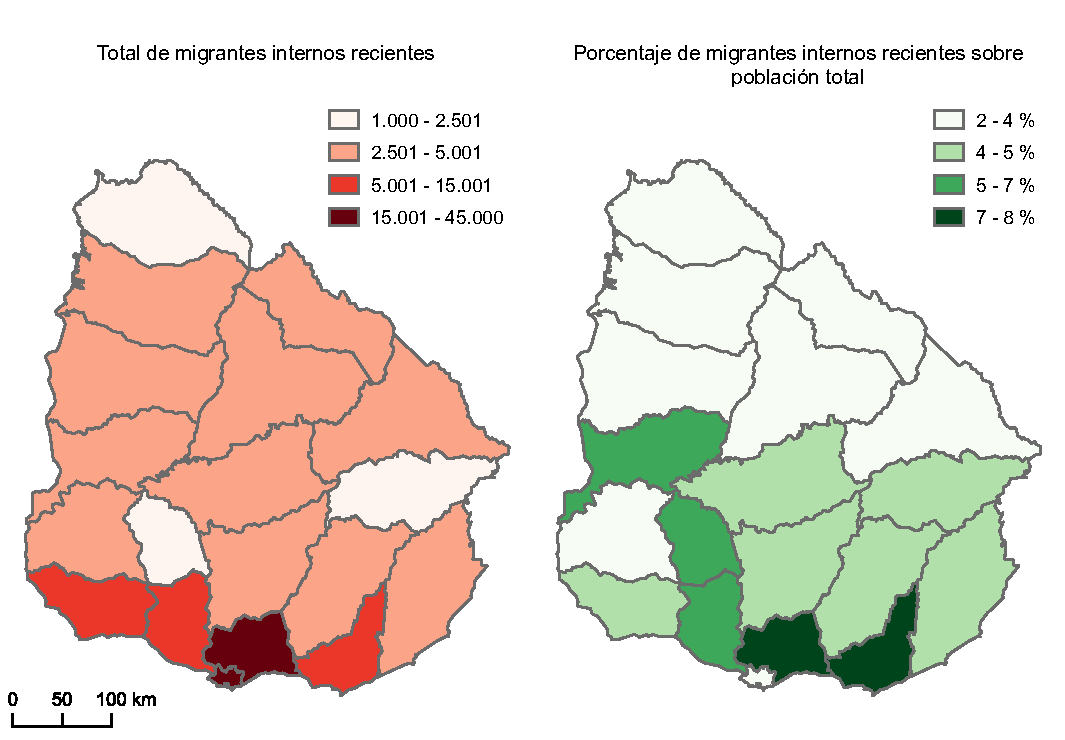
\includegraphics{./tex2pdf.-8c1f0593c1a83dbe/0fa4e601e9e3005ce60a7e916adf7e03dbd16ccd.pdf}
\caption{Migrantes internos recientes según el Censo
2011.}\label{fig:mapa_gemelo}
}
\end{figure}

El rol de Montevideo como receptor se puede vincular a la histórica
concentración de servicios en la capital (Bengochea, 2011), así como a
la concentración de actividad económica en general. El departamento de
Canelones también figura como atractor, y en parte se puede asociar a la
metropolización de la ciudad de Montevideo, es decir la expansión de su
``mancha urbana'' hacia el este, incorporando la zona costera de
Canelones (Ciudad de la Costa), como proceso de suburbanización
(D'Angelo, 2016; Folgar, 2005; Hernández, 1999).

Dicho proceso puede ser constado analizando las principales localidades
de destino de los migrantes internos que anteriormente residían en
Montevideo. Tal cual se constata en las~fig.~\ref{fig:mig_ori_mvo}
y~fig.~\ref{fig:mig_ori_mvo_zoom} el destino de preferencia es el área
metropolitana en primer lugar, en particular la costa de Canelones,
seguido de otras localidades costeras.

\begin{figure}
\hypertarget{fig:mig_ori_mvo}{%
\centering
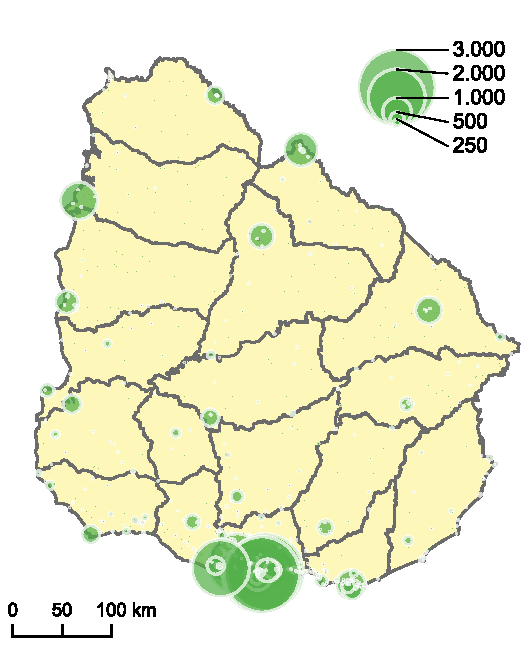
\includegraphics{./tex2pdf.-8c1f0593c1a83dbe/b9bc0fc10fd24a0e7eba94d94096c420d1bf6fa5.pdf}
\caption{Migrantes internos con origen en
Montevideo}\label{fig:mig_ori_mvo}
}
\end{figure}

Los 7 principales destinos corresponden a localidades del área
metrpolitana, y suman el 27\% de las personas migrantes interna con
origen den Montevideo.

\begin{figure}
\hypertarget{fig:mig_ori_mvo_zoom}{%
\centering
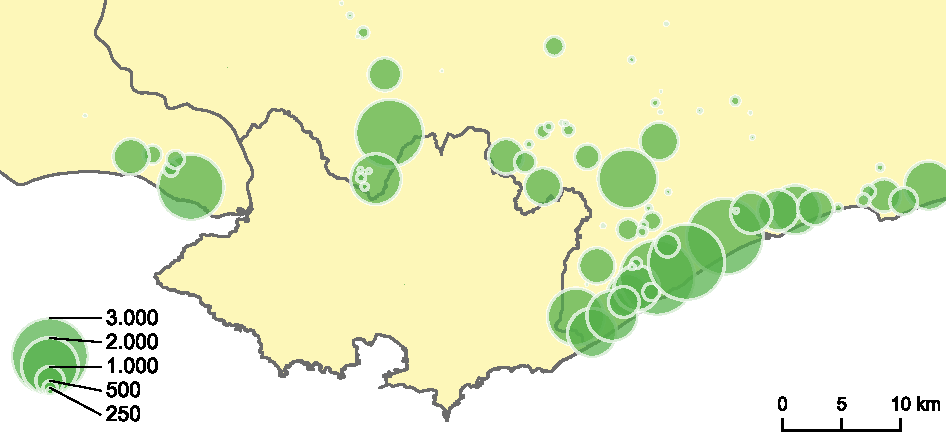
\includegraphics{./tex2pdf.-8c1f0593c1a83dbe/793a57bf2535638b71297054eae27fd13945f2db.pdf}
\caption{Migrantes internos con origen en Montevideo, zoom a área
metropolitana de Montevideo}\label{fig:mig_ori_mvo_zoom}
}
\end{figure}

En el mismo sentido, considerando las localidades del área metropolitana
como una entidad conjunta que aglomera partes de Canelones y San José
(Ciudad del Plata), el resultado del destino de los migrantes recientes
con orígen en Montevideo se puede apreciar en la~tabla~\ref{tbl:mig_am}.

\hypertarget{tbl:mig_am}{}
\begin{longtable}[]{@{}lrr@{}}
\caption{\label{tbl:mig_am}Migrantes recientes con origen en Montevideo,
por departamentos y area metropolitana de Montevideo.}\tabularnewline
\toprule
Entidad geográfica & personas & porcentaje\tabularnewline
\midrule
\endfirsthead
\toprule
Entidad geográfica & personas & porcentaje\tabularnewline
\midrule
\endhead
Área metropolitana & 32750 & 58.45\tabularnewline
Artigas & 894 & 1.6\tabularnewline
Canelones (no A.M.) & 1989 & 3.55\tabularnewline
Cerro Largo & 1355 & 2.42\tabularnewline
Colonia & 2015 & 3.6\tabularnewline
Durazno & 930 & 1.66\tabularnewline
Flores & 339 & 0.61\tabularnewline
Florida & 886 & 1.58\tabularnewline
Lavalleja & 746 & 1.33\tabularnewline
Maldonado & 3830 & 6.84\tabularnewline
Paysandú & 1059 & 1.89\tabularnewline
Río Negro & 821 & 1.47\tabularnewline
Rivera & 1626 & 2.9\tabularnewline
Rocha & 1211 & 2.16\tabularnewline
Salto & 1480 & 2.64\tabularnewline
San José (no A.M.) & 921 & 1.64\tabularnewline
Soriano & 1117 & 1.99\tabularnewline
Tacuarembó & 1329 & 2.37\tabularnewline
Treinta y Tres & 730 & 1.3\tabularnewline
Total & 56028 & 100\tabularnewline
\bottomrule
\end{longtable}

\textbf{Esta realidad plantea un debate: ¿es adecuado considerar esos
movimientos como migraciones internas o sería más preciso categorizarlas
como simples cambios de residencia?}

Aunque Montevideo sea un atractor relevante en números absolutos, si
atendemos al porcentaje de población migrante interna con respecto a la
población total de cada departamento, Canelones y Maldonado son los
departamentos que lideran. \textbf{En el caso de Maldonado, se puede
atribuir al dinamismo económico derivado de la actividad turística, así
como del sector de la construcción.}

\textless{}--- buscar cita \textgreater{}---

El grupo de migrantes internos puede ser dividido en tres subgrupos
(Bengochea, 2011), que para el presente análisis denominaremos grupo 1,
2 y 3:

\begin{itemize}
\item
  \textbf{Grupo 1}: 42.444 personas con origen en el interior del país
  pero residentes el Montevideo.
\item
  \textbf{Grupo 2}: 58.655 personas migrantes con origen en Montevideo
  pero residentes en el Interior del país.
\item
  \textbf{Grupo 3}: 47.660 personas con origen y residencia en el
  interior, pero en departamentos distintos.
\end{itemize}

A continuación se presentarán diversos indicadores referidos a dichos
tres grupos, para facilitar su carcterización.

\hypertarget{estructura-de-la-poblaciuxf3n}{%
\subsection{Estructura de la
población}\label{estructura-de-la-poblaciuxf3n}}

\hypertarget{distribuciuxf3n-por-sexo}{%
\subsubsection{Distribución por sexo}\label{distribuciuxf3n-por-sexo}}

El índice de masculinidad para el grupo 1 es de 80 hombres por cada 100
mujeres, para el grupo 2 de 92.4 y para el grupo tres es de 102.2
hombres por cada 100 mujeres. Dichos datos se presentan en forma gráfica
en la~fig.~\ref{fig:barras_mascul}.

\begin{figure}
\hypertarget{fig:barras_mascul}{%
\centering
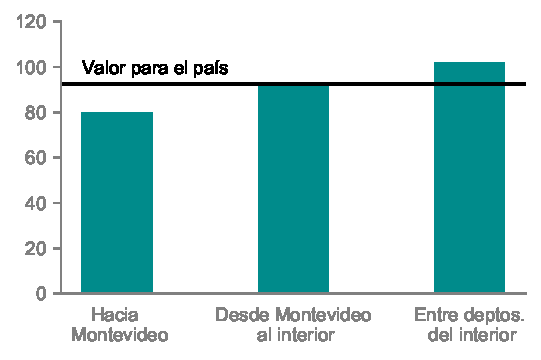
\includegraphics{./tex2pdf.-8c1f0593c1a83dbe/cac7dafaea377c79e54c748ede54da28c58dbdef.pdf}
\caption{Índice de masculinidad (mujeres cada 100 hombres) para el total
de personas y para los subconjuntos de migrantes internos
recientes.}\label{fig:barras_mascul}
}
\end{figure}

Los valores mencionados indican la mayor proporción de mujeres en el
grupo 1, posiblemente asociado a la matrícula universitaria, ya que esta
se caracteriza por ser feminizada (Bengochea, 2011; Universidad de la
República, 2013). Además la oferta educativa de la Universidad de la
República, la principal universidad del país y de carácter público, se
concentra en Montevideo (el impulso a la descentralización de la Udelar
fue posterior a la realización del Censo 2011). Por el contrario, el
grupo 3 presenta una leve masculinización con respecto a la mediana del
país, posiblemente asociado a migraciones por trabajo relacionadas al
sector agropecuario o al medio rural.

La~fig.~\ref{fig:porcen_sexo} ilustra la distribución por sexo dentro de
los grupos, coincidiendo con las apreciaciones anteriores.

\begin{figure}
\hypertarget{fig:porcen_sexo}{%
\centering
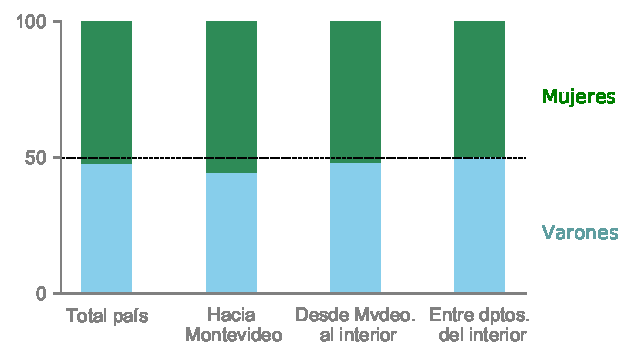
\includegraphics{./tex2pdf.-8c1f0593c1a83dbe/f6bf7303e4a1f285e872a927fdce827108d9d4d7.pdf}
\caption{Distribución por sexo para el total de personas y para los
subconjuntos de migrantes internos recientes.}\label{fig:porcen_sexo}
}
\end{figure}

\hypertarget{composiciuxf3n-por-edades}{%
\subsubsection{Composición por edades}\label{composiciuxf3n-por-edades}}

Atendiendo a la composición por edades, las \textbf{edades medianas}
para cada grupo son de \textbf{23, 32 y 28 años respectivamente}, en
tanto el valor para el país es de 34 años. Es decir que son poblaciones
levemente más jóvenes, con excepción del grupo 1, que es
considerablemente más joven que el total de la población.

\begin{figure}
\hypertarget{fig:edad_mediana}{%
\centering
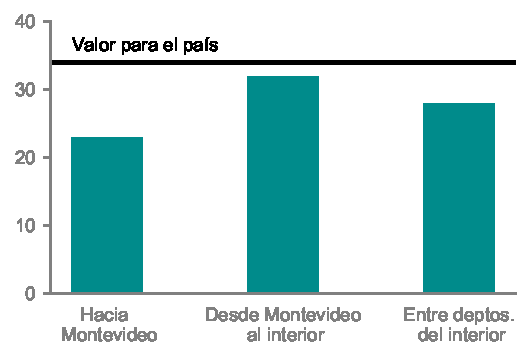
\includegraphics{./tex2pdf.-8c1f0593c1a83dbe/8922d0cd3e2baebc1841ef9a39ff35a49fdb43fc.pdf}
\caption{Edades medianas para el total de personas y para los
subconjuntos de migrantes internos recientes.}\label{fig:edad_mediana}
}
\end{figure}

La distribución por grupos de edades en la~fig.~\ref{fig:grupos_edades}
evidencia dicha estructura, con mayor concentración de la población en
el tramo de las personas económicamente activas en los grupos migrantes,
siendo el grupo 1 en el cual esta población tiene mayor presencia.

\begin{figure}
\hypertarget{fig:grupos_edades}{%
\centering
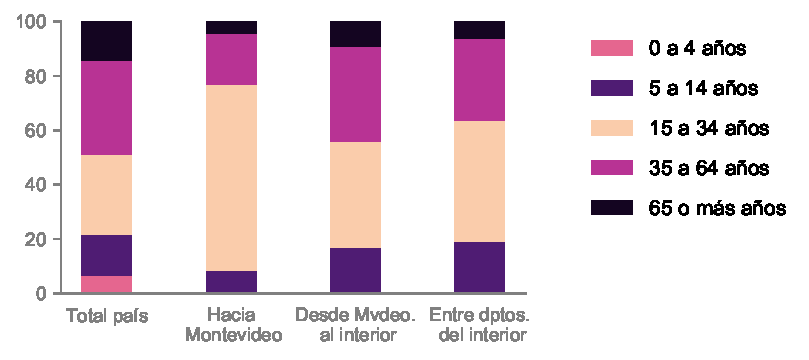
\includegraphics{./tex2pdf.-8c1f0593c1a83dbe/7a56c14120518b80c5308689d935792c3446129b.pdf}
\caption{Distribución por grupos de edades.}\label{fig:grupos_edades}
}
\end{figure}

La~fig.~\ref{fig:distri_edades} presenta la distribución por edades,
brindando un poco más de detalle sobre la conformación estructura de los
grupos. El grupo 1 presenta un pico en el tramo 18-25 años, coincidente
con la edad característica de los estudiantes universitarios, en tanto
el grupo 2 presenta más concentración en el grupo 25-35 años. El grupo 3
presenta concentración en las edades 18-25 años, pero también abarca
personas en el grupo 25-35 años. Los grupos 2 y 3 también están
conformados por niños y jóvenes, por oposición al grupo 1; pero el grupo
2 presenta mayor proporción de niños y menor de jóvenes, lo cual estaría
indicando que refiere a hogares de parejas en el tramo 25-35 años, con
niños.

\begin{figure}
\hypertarget{fig:distri_edades}{%
\centering
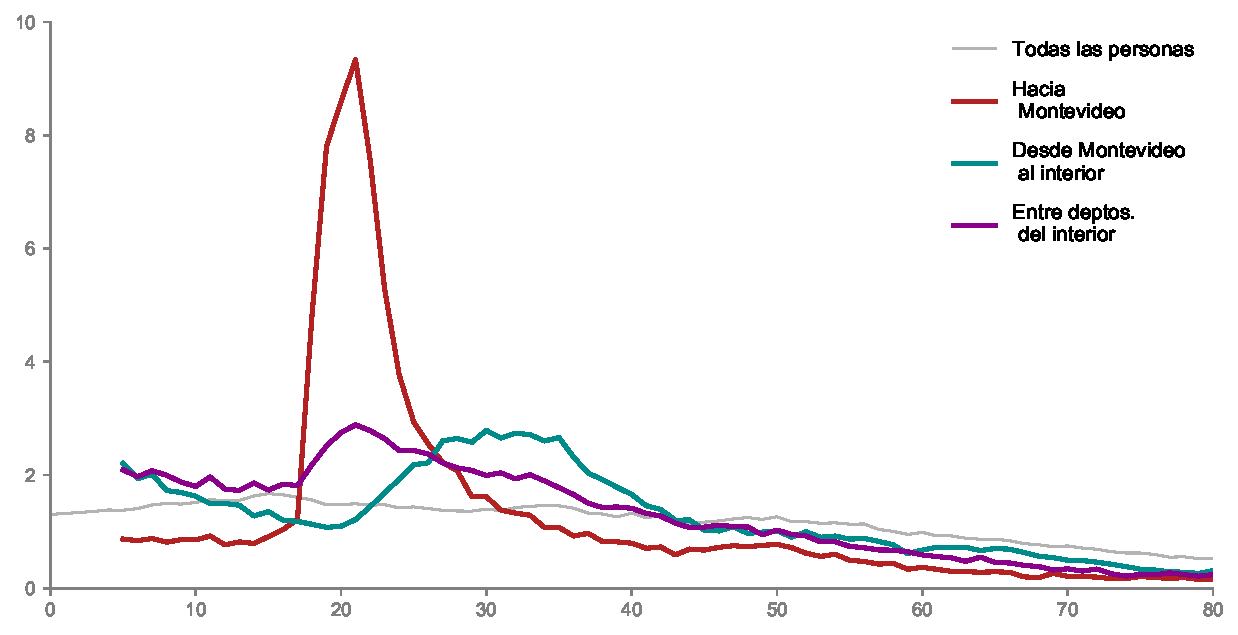
\includegraphics{./tex2pdf.-8c1f0593c1a83dbe/2cc2f92e9c80908b688429b7d753e4b33361e702.pdf}
\caption{Distribución de edades, porcentaje dentro de cada
grupo.}\label{fig:distri_edades}
}
\end{figure}

\hypertarget{piruxe1mides-de-poblaciuxf3n}{%
\subsubsection{Pirámides de
población}\label{piruxe1mides-de-poblaciuxf3n}}

La distribución por sexo y tramos de edad se puede integrar en pirámides
de población, que dan cuenta de la estructura de la población en forma
más abarcadora. La pirámide de los migrantes internos, como es de
esperar, concentra población en las edades económicamente activas en
comparación con la pirámide de todo el conjunto de población censada. A
su vez, es una población más feminizada, sobre todo en los tramos de
edad entre 15 y 34 años.

\begin{figure}
\centering
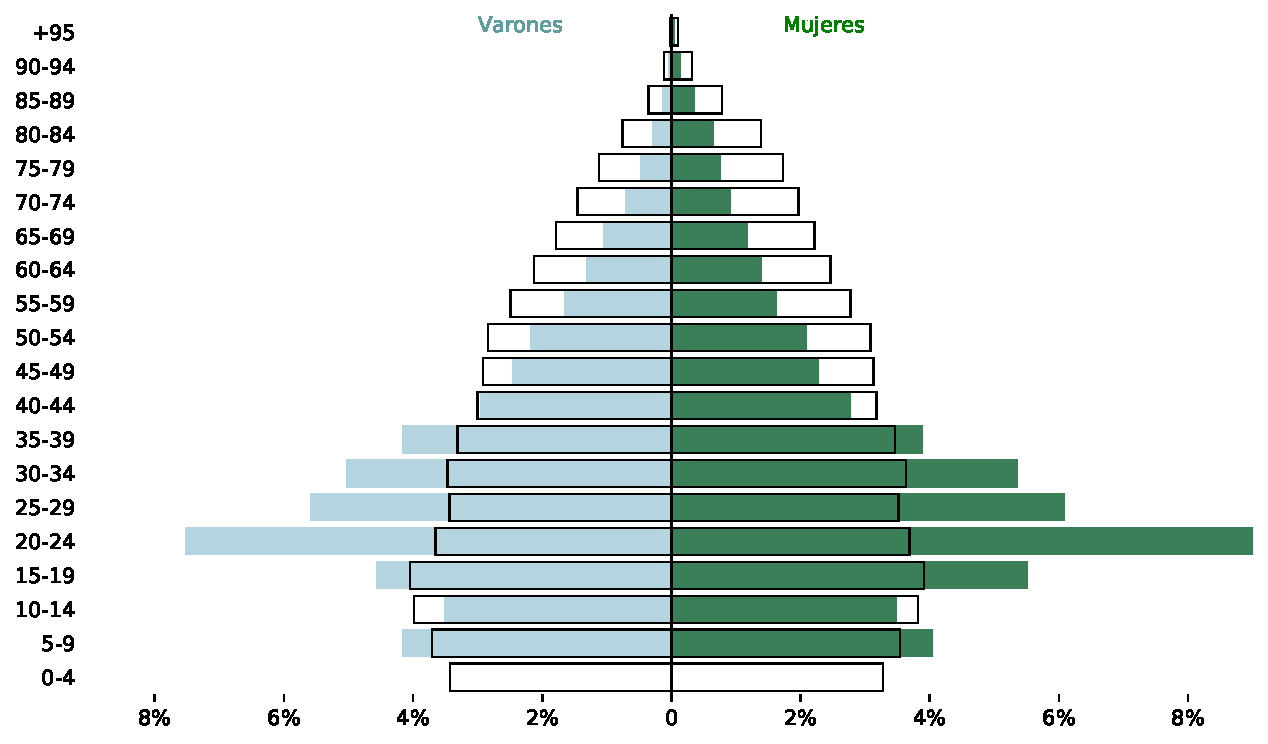
\includegraphics{./tex2pdf.-8c1f0593c1a83dbe/1d0238859672b630db570be11ac54a39ca2696a0.pdf}
\caption{Pirámides de población del total de población y de los
migrantes internos.}
\end{figure}

Comparando las pirámides de los grupos 1, 2 y 3 en
la~fig.~\ref{fig:piramides_mig_rec}, se pueden identificar visualmente
varias de las afirmaciones hechas con anterioridad. En particular la
estructura de la pimrámide correspondiente al grupo 2, que estará
indicando hogares conformados por parejas de mediana edad y con niños,
posiblemente muchos refieran a movimientos desde Montevideo hacia la
costa de Canelones, en el marco del proceso de metropolización
anteriomente mencionado.

\begin{figure}
\hypertarget{fig:piramides_mig_rec}{%
\centering
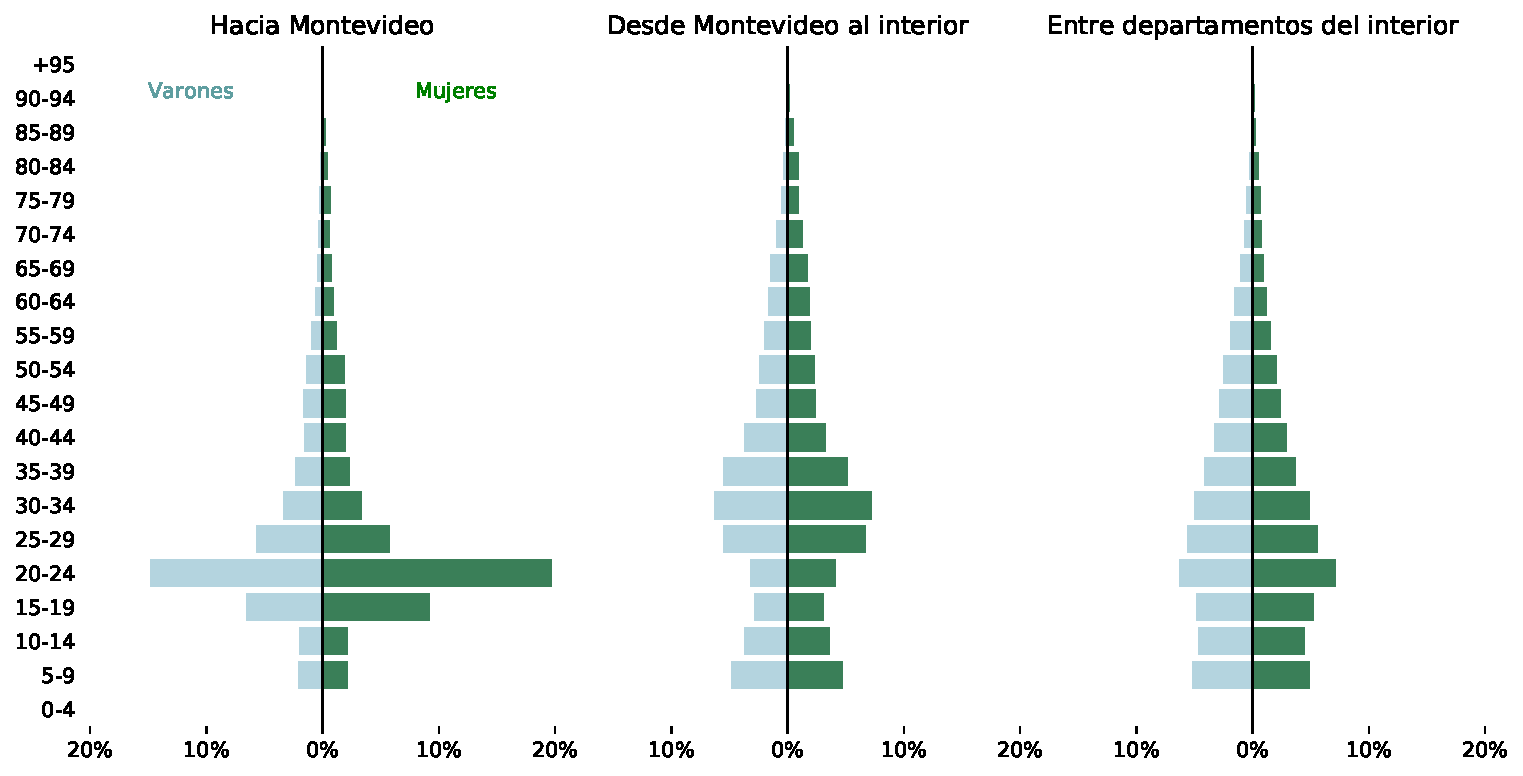
\includegraphics{./tex2pdf.-8c1f0593c1a83dbe/9df7a052b593b5eba7775a004f9848c10cc3b554.pdf}
\caption{Pirámides de población migrantes internos desde el Interior
hacia Montevideo, desde Montevideo al interior o entre departamentos del
interior.}\label{fig:piramides_mig_rec}
}
\end{figure}

Para profundizar en las diferencias del grupo 1 con el resto de los
grupos, se analiza el promedio de personas que componen los hogares
dentro de los cuales hay al menos una persona migrante. En general los
hogares que conforman el grupo 1 tienen menos integrantes, y los del
grupo 3 tienen más. Se excluyen de estos cálculos a los hogares
colectivos (pensiones, hogares estudiantiles, cuarteles miitares,
prisiones, etc.)

\begin{figure}
\hypertarget{fig:prom_perso_hogar}{%
\centering
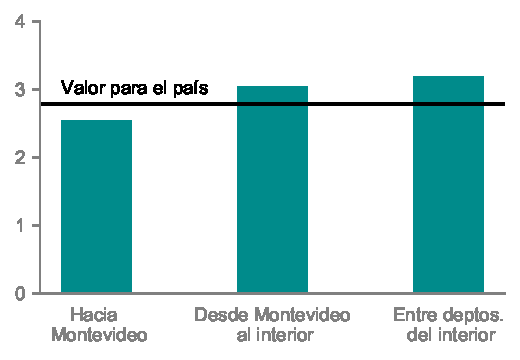
\includegraphics{./tex2pdf.-8c1f0593c1a83dbe/c6ede563c6d7a200b20028927b4edd7e49ad66bd.pdf}
\caption{Promedio de personas por hogar, excluyendo hogares
colectivos}\label{fig:prom_perso_hogar}
}
\end{figure}

En el mismo sentido, el porcentaje de personas migrantes internas
viviendo en hogares colectivos, como ser hogares estudiantiles, es mucho
mayor en el grupo 1.

\begin{figure}
\hypertarget{fig:viv_colectivas}{%
\centering
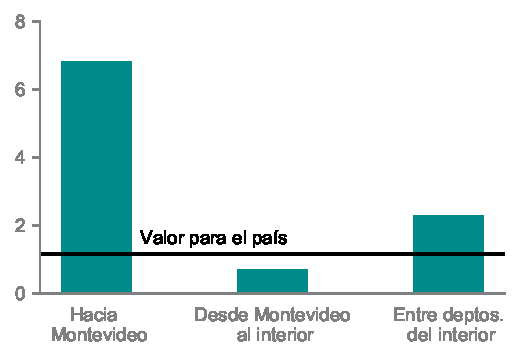
\includegraphics{./tex2pdf.-8c1f0593c1a83dbe/8480b873ee7013ad523b67bbe5cc238a5ff00ee5.pdf}
\caption{Porcentaje de personas viviendo en hogares
colectivos}\label{fig:viv_colectivas}
}
\end{figure}

\hypertarget{nivel-educativo}{%
\subsection{Nivel educativo}\label{nivel-educativo}}

Otro factor de interés para la caracterización es el nivel educativo de
la población migrante interna. En lo que refiere a la asistencia a un
centro educativo, el grupo 1 se destaca por quienes declaran asistir
tanto a centros públicos como privados.

\begin{figure}
\centering
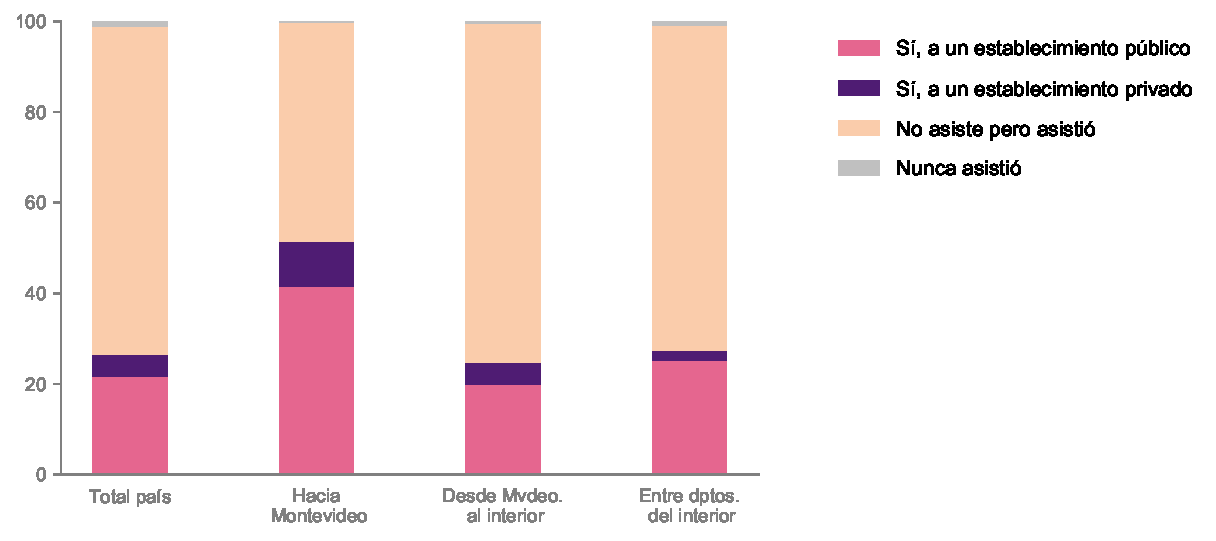
\includegraphics{./tex2pdf.-8c1f0593c1a83dbe/14d3c1fbe2546fa9f3845f99c60d49f9d2180e27.pdf}
\caption{Asistencia a centros educativos.}
\end{figure}

El grupo 1 también se diferencia en cuánto al nivel educativo actual en
el momento del censo, con la preeminencia de aquellos cursando estudios
terciarios, principalmente universitarios.

\begin{figure}
\centering
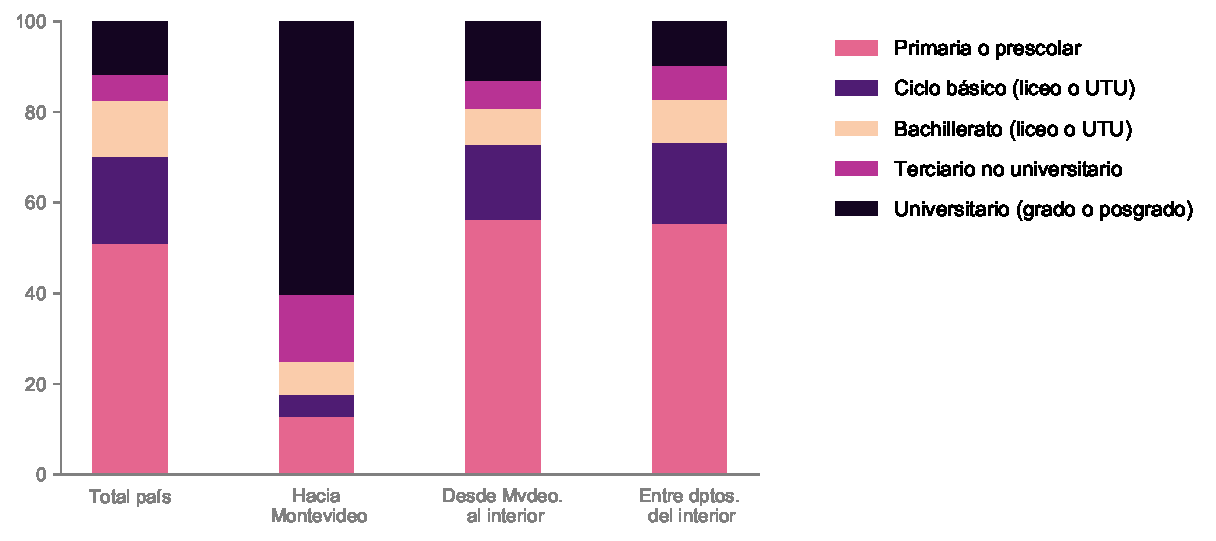
\includegraphics{./tex2pdf.-8c1f0593c1a83dbe/b566f3c7e0aa02793c11dfed1ace2ea686608e1c.pdf}
\caption{Nivel educativo actual.}
\end{figure}

En cuanto al nivel educativo más alto alcanzado, se puede apreciar que
los grupos 1 y 2 tienen una distribución prácticamente similar similar,
en tanto el grupo 3 presenta menor porcentaje de personas que han
alcanzado los estudios universitarios, aún en comparación con los
porcentajes de toda la población.

\begin{figure}
\centering
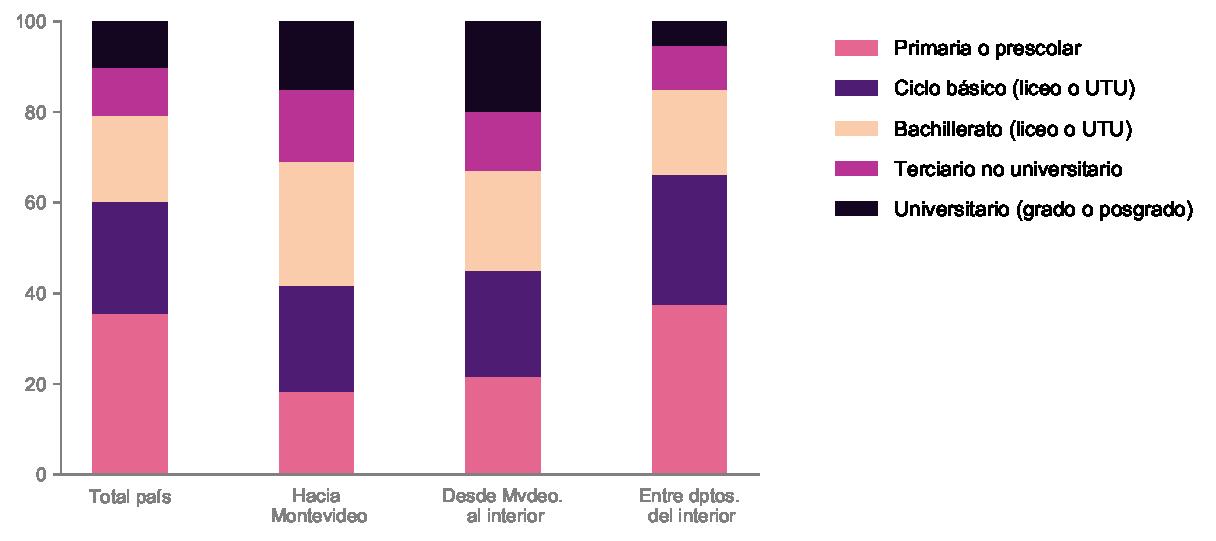
\includegraphics{./tex2pdf.-8c1f0593c1a83dbe/f71a7e5209d4cb5db71480e46fca3e283c9632b3.pdf}
\caption{Máximo nivel educativo alcanzado.}
\end{figure}

\newpage

\hypertarget{factores-asociados-a-las-migraciones-internas}{%
\subsection{Factores asociados a las migraciones
internas}\label{factores-asociados-a-las-migraciones-internas}}

El estudio de las migraciones internas está relacionado a los procesos
de migración rural-urbano, propios de las sociedades pre-transición
demográfica. Sin embargo, Uruguay vivió la transición demográfica en
forma temprana en comparación con sus pares latinoamericanos, y presenta
un alto grado de urbanización, con un medio rural escasamente poblado.

Existen varias razones que pueden estar detrás del interés de migrar de
una personas y la concreción de dicho movimiento, a continuación se
analizan algunos de los factores que según la literatura se asocian al
proceso migratorio.

La razón más general, aplicada especialmente a las migraciones no
forzadas, es la búsqueda de un ingreso mayor, que aplica con mayor
intensidad a los jóvenes (Lucas, 1997).

Weidlich et. al (1988) identificaron cuatro factores clave en la
migración interna para el caso de la Alemania Federal de posguerra,
utilizando análisis de regresión:

\begin{itemize}
\tightlist
\item
  Ingreso real \emph{per cápita}
\item
  Puesto de trabajo vacantes
\item
  Índice de estructura de inversiones
\item
  Número de personas empleadas
\end{itemize}

Algunas investigaciones de los determinantes económicos y no económicos
de la migración interna en Estados Unidos (Cebula, 2005; Cebula y
Alexander, 2006) identifican variables asociadas a la migración
interestatal. Algunas variables están relacionadas con la calidad de
vida (incidencia de luz solar, número de crímenes violentos por 100.000
habs., superficie de parques estatales por 100.000 habs., número de
sitios de deposición final de residuos peligrosos, temperatura máxima
diaria en enero por estado). Por otro lado identifican como
significativo el costo de vida en destino y la variable ``ingresos
esperados en destino'' (el ingreso \emph{per cápita} multiplicado por la
tasa de empleo, ambos factores según datos de 1999).

En un estudio de migracion interprovincial en Turquía (Filiztekin y
Gökhan, 2008), se identificaron las siguientes variables con incidencia
estadísticamente significativa (al 1\%) sobre los flujos migratorios:

\begin{itemize}
\tightlist
\item
  Distancia entre provincias
\item
  Tasa de desempleo en origen y destino
\item
  Proporción de personas jóvenes (entre 12 y 25 años)
\item
  Promedio de años de escolarización en la provincia de origen
\item
  Stock de migrantes anteriores entre las provincias i y j
\item
  Variables dummy para indicar migración entre regiones o migración
  hacia Estanbul
\end{itemize}

Existen diversas investigaciones al respecto, que aún quedan pendientes
de análisis para el presente trabajo.

\hypertarget{primera-aplicaciuxf3n-de-un-modelo-de-interaciuxf3n-espacial}{%
\section{Primera aplicación de un modelo de interación
espacial}\label{primera-aplicaciuxf3n-de-un-modelo-de-interaciuxf3n-espacial}}

A continuación se presenta una primera aplicación de modelos de
interacción espacial, basada en los datos del Censo INE 2011 (INE,
2011c), publicados en la página web del Instituto. Como capas de
información geográfica se accedió a las capas de polígonos de
departamentos y de puntos de localidades del INE, identificando las
capitales departamentales en esta última capa (INE, 2011b).

Se incluye una matriz de distancias entre cada centro medio de
población, calculada con la API Google Distance Matrix (Google, 2017a),
que consta de distancias siguiendo el camino recomendado por la API
Google Maps (Google, 2017b), por la red de caminería, entre el centro
medio de población de cada departamento, obteniendo una matriz con 342
valores ((19x19)-19).

Se prefirió usar el centro medio de población, en detrimento del
centroide o la capital departamental. El centro medio de población se
calcula transfiriendo el conteo de habitantes del segmento censal al
centroide de dicho segmento y luego aplicando la siguiente fórmula (Burt
et~al., 2009):

\[
\overline{X}_w=\frac{\sum_{i=1}^{n}w_{i}X_{i}}{\sum_{i=1}^{n} w_{i}}
\]

\[
\overline{Y}_w=\frac{\sum_{i=1}^{n}w_{i}Y_{i}}{\sum_{i=1}^{n} w_{i}}
\]

En este caso el ``peso'' (\(w\)) sería la población, en tanto que ``x''
e ``y'' son las coordenadas cartográficas de cada centroide. De esta
forma se obtiene un par de coordenadas para cada departamento, que
representa ese centro medio.

\begin{figure}
\centering
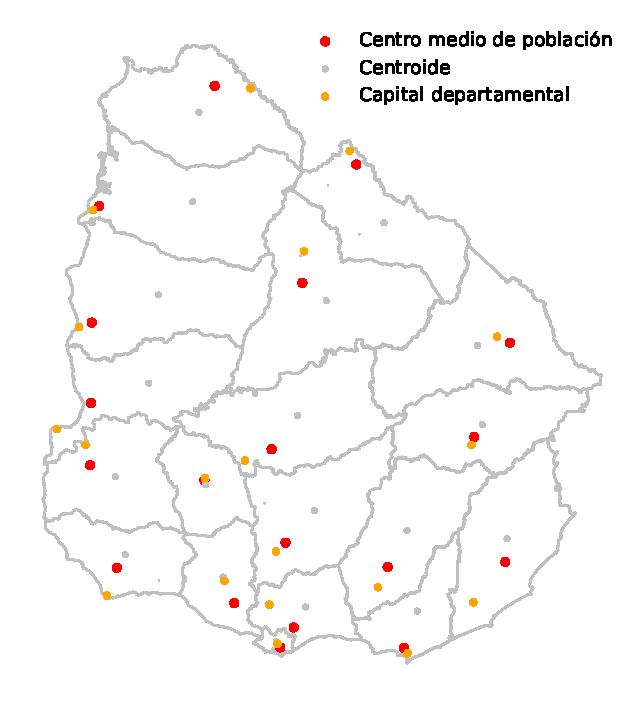
\includegraphics{./tex2pdf.-8c1f0593c1a83dbe/1e1ebe914247a06bc0fb87bbc6d2d9c0f8ecab24.pdf}
\caption{Mapa de centroides, capitales departamentales y centro medio de
población calculado según las fórmulas mencionadas.}
\end{figure}

Dada la menor complejidad, se comienza por el análisis de los flujos
entre departamentos.

Aquí surge una primera complejidad, asociada a los ya mencionados
solapamientos entres las movilidades pendulares, las residenciales y las
migraciones, y refiere a la operacionalización del concepto de migrante
interno.

Según la información disponible en Censo INE (INE, 2011c), el criterio
más adecuado sería usar los datos relevados en la pregunta ``lugar de
residencia 5 años antes'', la cual puede tomar los siguientes valores:

\begin{itemize}
\tightlist
\item
  Lugar de residencia 5 años antes (variable ``PERMI07'') con valores:

  \begin{itemize}
  \tightlist
  \item
    ``2'' (en otra localidad o paraje de este departamento)
  \item
    ``3'' (en otro departamento)
  \end{itemize}
\end{itemize}

Se encuentran al menos dos limitaciones. En primer lugar se excluyen
habitantes de zonas rurales de población dispersa, es decir aquellas sin
localidad INE asignada. Para estudiar las migraciones referidas al
ámbito rural, habría que tomar otra estrategia de abordaje. EN segundo
lugar, residir en otro departamento con anterioridad no necesariamente
debería ser una migración. Por ejemplo, una hogar con residencia en
Ciudad del Plata o Ciudad de la Costa, cuya residencia 5 años antes era
en Montevideo, ¿migró o simplemente cambió de residencia?. Aquí es donde
la distancia del movimiento realizado puede servir como variable
auxiliar para determinar a que categoría corresponde.

Del procesamiento inicial de la variable ``Lugar de residencia 5 años
antes'', se obtiene una tabla que contiene un departamento de origen,
uno de destino y una cantidad de personas que declaran haber vivido
antes en el departamento de ``origen'', habiendo sido relevadas en el
departamento de ``destino'' al momento de la aplicación del formulario
censal.

\begin{longtable}[]{@{}rrr@{}}
\caption{Tabla de díadas orígen-destino, referida por códigos INE de
departamentos.}\tabularnewline
\toprule
Cod. dpto. origen & Cod. dpto. destino & Pers. Migrantes\tabularnewline
\midrule
\endfirsthead
\toprule
Cod. dpto. origen & Cod. dpto. destino & Pers. Migrantes\tabularnewline
\midrule
\endhead
1 & 2 & 914\tabularnewline
1 & 3 & 33127\tabularnewline
1 & 4 & 1387\tabularnewline
1 & 5 & 2100\tabularnewline
1 & 6 & 982\tabularnewline
\bottomrule
\end{longtable}

Esos datos también pueden ser representados como una matriz, en la cual
se utilizan los códigos INE de departamentos como identificadores en el
eje X, para una representación adecuada.

\newpage
\begin{landscape}
\begin{table}
\centering
\caption{Matriz de movimientos entre departamentos (Censo INE 2011).}
\begin{tabular}{lp{0.7cm}p{0.7cm}p{0.7cm}p{0.7cm}p{0.7cm}p{0.7cm}p{0.7cm}p{0.7cm}p{0.7cm}p{0.7cm}p{0.7cm}p{0.7cm}p{0.7cm}p{0.7cm}p{0.7cm}p{0.7cm}p{0.7cm}p{0.7cm}p{0.7cm}p{0.7cm}}
\toprule
depto\_destino &      1 &     2 &      3 &     4 &     5 &     6 &     7 &     8 &     9 &     10 &    11 &    12 &    13 &    14 &    15 &    16 &    17 &    18 &    19 &   Total \\
depto\_origen &        &       &        &       &       &       &       &       &       &        &       &       &       &       &       &       &       &       &       &         \\
\midrule
Mvdeo.       &      0 &   914 &  33127 &  1387 &  2100 &   982 &   378 &  1026 &   825 &   3914 &  1075 &   886 &  1665 &  1266 &  1547 &  4209 &  1173 &  1421 &   760 &   58655 \\
Artigas      &   2395 &     0 &    536 &    20 &   167 &    33 &    21 &    40 &    15 &    472 &   200 &    57 &   146 &    47 &   794 &    92 &    24 &   100 &     5 &    5164 \\
Can.         &  11162 &    74 &      0 &   274 &   422 &   223 &    82 &   670 &   403 &   1345 &   148 &   154 &   320 &   360 &   159 &   908 &   154 &   251 &   124 &   17233 \\
C. Largo     &   1805 &    15 &    435 &     0 &    63 &    67 &     5 &    73 &   131 &    810 &    61 &    41 &   145 &    95 &    19 &    49 &    34 &   135 &   476 &    4459 \\
Colonia      &   2690 &    28 &    366 &    20 &     0 &    63 &    69 &    53 &    19 &    309 &    71 &    88 &    34 &    35 &    68 &   269 &   513 &    34 &    23 &    4752 \\
Durazno      &   1610 &    32 &    466 &    64 &    70 &     0 &   149 &   404 &    67 &    198 &    59 &    62 &    42 &    61 &    28 &   124 &    32 &   212 &    77 &    3757 \\
Flores       &    735 &     2 &    162 &    13 &    86 &    90 &     0 &    76 &     5 &     79 &    30 &    36 &    10 &    13 &    17 &   116 &    85 &    29 &    14 &    1598 \\
Florida      &   1420 &    13 &    892 &    37 &   107 &   307 &    84 &     0 &   163 &    310 &    47 &    30 &    46 &    62 &    19 &   321 &    51 &    68 &    64 &    4041 \\
Lavalleja    &   1264 &     7 &    446 &    64 &    39 &    29 &    17 &   138 &     0 &    936 &    28 &    11 &    25 &   150 &    15 &    45 &    11 &    45 &   221 &    3491 \\
Maldonado    &   2333 &    46 &    862 &   208 &   196 &    75 &    58 &   121 &   407 &      0 &    95 &    95 &   117 &   535 &    98 &   131 &   110 &    71 &   259 &    5817 \\
Paysandú     &   2096 &    75 &    434 &    35 &   151 &    55 &    29 &    57 &    37 &    420 &     0 &   640 &    66 &    50 &   480 &   116 &    98 &   229 &    25 &    5093 \\
R. Negro     &   1219 &    30 &    316 &    20 &   176 &    54 &    77 &    27 &    15 &    223 &   516 &     0 &    54 &    48 &   133 &   107 &   270 &    89 &     9 &    3383 \\
Rivera       &   2390 &   102 &    584 &   162 &    77 &    50 &    22 &    63 &    49 &    227 &   143 &    36 &     0 &    46 &   120 &    99 &    25 &   546 &    57 &    4798 \\
Rocha        &   1435 &     8 &    407 &    59 &    49 &    18 &     7 &    45 &   130 &    952 &    32 &    30 &    17 &     0 &    29 &    45 &    18 &    21 &   162 &    3464 \\
Salto        &   2481 &   380 &    543 &    18 &   134 &    14 &    20 &    48 &    20 &    484 &   564 &   161 &    97 &    38 &     0 &    99 &    75 &   166 &     8 &    5350 \\
San José     &   1852 &    15 &    689 &    31 &   452 &    59 &   122 &   252 &    44 &    230 &    59 &    55 &    32 &    47 &    30 &     0 &   112 &    53 &    23 &    4157 \\
Soriano      &   1922 &     9 &    293 &    12 &  1053 &    57 &    90 &    40 &    33 &    335 &   181 &   372 &    18 &    46 &    98 &   147 &     0 &    41 &    16 &    4763 \\
Tacuarembó   &   2611 &    50 &    596 &   168 &    79 &   304 &    79 &    92 &    50 &    363 &   261 &   134 &   421 &    35 &   174 &    88 &    72 &     0 &    32 &    5609 \\
T. y Tres    &   1024 &    10 &    259 &   409 &    41 &    91 &     2 &    58 &   172 &    776 &    16 &    16 &    23 &   174 &    13 &    28 &    25 &    38 &     0 &    3175 \\
Total        &  42444 &  1810 &  41413 &  3001 &  5462 &  2571 &  1311 &  3283 &  2585 &  12383 &  3586 &  2904 &  3278 &  3108 &  3841 &  6993 &  2882 &  3549 &  2355 &  148759 \\
\bottomrule
\end{tabular}
\end{table}

\end{landscape}

Siguiendo la estructura de datos presentada anteriormente (tabla de
díadas origen-destino), se construye un conjunto de datos conteniendo la
siguiente información para cada díada de departamentos:

\begin{itemize}
\tightlist
\item
  Totales de personas que declaran haber vivido antes en el departamento
  de origen
\item
  La población total en origen y destino
\item
  El PBI en el departamento de destino y el logaritmo de dicho valor
  (OPP, 2016)
\item
  La distancia entre cada centro medio de población y el logaritmo de
  dicho valor
\end{itemize}

\hypertarget{modelo-de-interacciuxf3n-espacial-restringido-en-origen}{%
\subsubsection{Modelo de interacción espacial restringido en
origen}\label{modelo-de-interacciuxf3n-espacial-restringido-en-origen}}

A continuación se presenta una primera aplicación del modelo restringido
en origen, seleccionando solo las variables ``logaritmo del PBI en
destino'' y ``logaritmo de la distancia''. El procesamiento es similar
al aplicado por (Dennett, 2018) y su adaptación al lenguaje de
programación Python (Lewis, 2018).

El modelo se define de la siguiente forma:

1 \[T_{ij} = A_{i}O_{i}W_{j}^{\alpha}d_{ij}^{-\beta}\]

dónde

2 \[O_{i} = \sum_{j}T_{ij}\]

3 \[A_{i} = \frac{1}{\sum_{j}W_{j}^{\alpha}d_{ij}^{-\beta}}\]

En el modelo restringido en origen \(O_{i}\) no tiene parámetro dado que
refiere valores conocidos. \(A_{i}\) es un factor de balance que refiere
a cada origen \(i\). Más específicamente \(A_{i}\) permite que la suma
de los valores estimados sea igual al total conocido \(O_{i}\)

La forma multiplicativa del modelo puede ser modificada, re-especificado
el modelo como un modelo de regresión de Poisson (Dennett, 2018). Para
ello se aplica el logaritmo al lado derecho de la ecuación, y asumiendo
que están logarítmicamente vinculados a la media con distribución de
Poisson (\(\lambda_{ij}\)) de la variable \(T_{ij}\), se obtiene

4
\[ \lambda_{ij} = \exp( \mu_{i} + \alpha \ln W_{j} - \beta \ln d_{ij} )\]

Reemplazamos la variable independiente (los estimados \(T_{ij}\)) por la
media de la distribución de Poisson \(\lambda_{ij}\), la cual se asume
como modelada por una combinación lineal de las variables del modelo.

En esta ecuación \(\mu_{i}\) es el equivalente al vector \(A_{i}O_{i}\),
pero en la terminología de una regresión log-lineal se pueden describir
como variables dummy. En la práctica, en el modelo de regresión
\(\mu_{i}\) será tomado como un predictor categórico, por ende en el
modelo de regresión de Poisson los valores de \(O_{i}\) son reemplazados
por un identificador categórico del origen, por ejemplo el código INE o
el nombre del departamento (Dennett, 2018).

El primer modelo se corrió con las variables departamento de destino,
logaritmo del PBI departamental en destino y logaritmo de la distancia.

\begin{center}
\begin{tabular}{lclc}
\toprule
\textbf{Dep. Variable:}                   &  personas\_mig   & \textbf{  No. Observations:  } &      342    \\
\textbf{Model:}                           &       GLM        & \textbf{  Df Residuals:      } &      321    \\
\textbf{Model Family:}                    &     Poisson      & \textbf{  Df Model:          } &       20    \\
\textbf{Link Function:}                   &       log        & \textbf{  Scale:             } &    1.0000   \\
\textbf{Method:}                          &       IRLS       & \textbf{  Log-Likelihood:    } &   -14973.   \\
\textbf{Date:}                            & Sat, 10 Apr 2021 & \textbf{  Deviance:          } &    27718.   \\
\textbf{Time:}                            &     12:05:55     & \textbf{  Pearson chi2:      } &  3.00e+04   \\
\textbf{No. Iterations:}                  &        6         & \textbf{                     } &             \\
\bottomrule
\end{tabular}
\begin{tabular}{lcccccc}
                                          & \textbf{coef} & \textbf{std err} & \textbf{z} & \textbf{P$> |$z$|$} & \textbf{[0.025} & \textbf{0.975]}  \\
\midrule
\textbf{nom\_depto\_orig[ARTIGAS]}        &       0.8906  &        0.075     &    11.948  &         0.000        &        0.745    &        1.037     \\
\textbf{nom\_depto\_orig[CANELONES]}      &       0.3788  &        0.069     &     5.491  &         0.000        &        0.244    &        0.514     \\
\textbf{nom\_depto\_orig[CERRO LARGO]}    &       0.5190  &        0.074     &     6.988  &         0.000        &        0.373    &        0.665     \\
\textbf{nom\_depto\_orig[COLONIA]}        &       0.1648  &        0.073     &     2.255  &         0.024        &        0.022    &        0.308     \\
\textbf{nom\_depto\_orig[DURAZNO]}        &      -0.0837  &        0.073     &    -1.140  &         0.254        &       -0.227    &        0.060     \\
\textbf{nom\_depto\_orig[FLORES]}         &      -1.0428  &        0.075     &   -13.842  &         0.000        &       -1.190    &       -0.895     \\
\textbf{nom\_depto\_orig[FLORIDA]}        &      -0.3389  &        0.073     &    -4.672  &         0.000        &       -0.481    &       -0.197     \\
\textbf{nom\_depto\_orig[LAVALLEJA]}      &      -0.3429  &        0.073     &    -4.688  &         0.000        &       -0.486    &       -0.200     \\
\textbf{nom\_depto\_orig[MALDONADO]}      &       0.2271  &        0.073     &     3.128  &         0.002        &        0.085    &        0.369     \\
\textbf{nom\_depto\_orig[MONTEVIDEO]}     &       2.5748  &        0.067     &    38.545  &         0.000        &        2.444    &        2.706     \\
\textbf{nom\_depto\_orig[PAYSANDU]}       &       0.5033  &        0.073     &     6.882  &         0.000        &        0.360    &        0.647     \\
\textbf{nom\_depto\_orig[RIO NEGRO]}      &      -0.0120  &        0.073     &    -0.164  &         0.870        &       -0.156    &        0.132     \\
\textbf{nom\_depto\_orig[RIVERA]}         &       0.7054  &        0.074     &     9.489  &         0.000        &        0.560    &        0.851     \\
\textbf{nom\_depto\_orig[ROCHA]}          &       0.0459  &        0.074     &     0.618  &         0.537        &       -0.100    &        0.192     \\
\textbf{nom\_depto\_orig[SALTO]}          &       0.7632  &        0.074     &    10.334  &         0.000        &        0.618    &        0.908     \\
\textbf{nom\_depto\_orig[SAN JOSE]}       &      -0.4887  &        0.072     &    -6.775  &         0.000        &       -0.630    &       -0.347     \\
\textbf{nom\_depto\_orig[SORIANO]}        &       0.2470  &        0.073     &     3.389  &         0.001        &        0.104    &        0.390     \\
\textbf{nom\_depto\_orig[TACUAREMBO]}     &       0.6533  &        0.074     &     8.878  &         0.000        &        0.509    &        0.798     \\
\textbf{nom\_depto\_orig[TREINTA Y TRES]} &      -0.0210  &        0.074     &    -0.283  &         0.777        &       -0.167    &        0.125     \\
\textbf{log\_pbi\_destino}                &       0.8527  &        0.002     &   355.615  &         0.000        &        0.848    &        0.857     \\
\textbf{log\_dist}                        &      -0.7834  &        0.003     &  -224.855  &         0.000        &       -0.790    &       -0.777     \\
\bottomrule
\end{tabular}
%\caption{Generalized Linear Model Regression Results}
\end{center}

De los resultados se desprende un parámetro \(\alpha\) relacionado a la
actractividad del destino con un valor de 0,8527.

El parámetro \(\beta\) relativo al decaimiento por la distancia es de
-0,7830. El coeficiente para cada origen es el valor registrado
\(A_{i}O_{i}\) para ese origen.

Se identifican cuatro departamentos para los cuales el modelo no
devuelve un p-valor mayor a 0,05: Durazno, Río Negro, Rocha y Treinta y
Tres (no podemos rechazar la hipótesis nula).

A partir de los parámetros calculados se procede a la estimación del
modelo restringido en origen. Los parámetros se insertan en la ecuación
nro. 4.

\[ \lambda_{ij} = \exp( \mu_{i} + 0,8527 ln W_{j}  + 0,7830 ln d_{ij} )\]

Se recuperan los valores \(\mu_{i}\) que el modelo devuelve para cada
departamento.

A continuación se presenta el resultado de la estimación del modelo en
forma de matriz.

\newpage
\begin{landscape}
\begin{table}
\centering
\caption{Matriz de movimientos entre departamentos estimada mediante SIM restringido en origen.}
\begin{tabular}{lp{0.7cm}p{0.7cm}p{0.7cm}p{0.7cm}p{0.7cm}p{0.7cm}p{0.7cm}p{0.7cm}p{0.7cm}p{0.7cm}p{0.7cm}p{0.7cm}p{0.7cm}p{0.7cm}p{0.7cm}p{0.7cm}p{0.7cm}p{0.7cm}p{0.7cm}p{0.7cm}}
\toprule
depto\_destino &      1 &     2 &      3 &     4 &     5 &     6 &     7 &     8 &     9 &    10 &    11 &    12 &    13 &    14 &    15 &    16 &    17 &    18 &    19 &   Total \\
depto\_origen &        &       &        &       &       &       &       &       &       &       &       &       &       &       &       &       &       &       &       &         \\
\midrule
Mvdeo.       &      0 &   484 &  29872 &   797 &  3397 &  1081 &   705 &  2378 &  1714 &  5034 &  1237 &  1285 &   769 &  1159 &   953 &  4712 &  1438 &   900 &   739 &   58654 \\
Artigas      &   1761 &     0 &    423 &   144 &   252 &   107 &    64 &   121 &    99 &   253 &   266 &   206 &   337 &   106 &   378 &   163 &   173 &   219 &    92 &    5164 \\
Can.         &  14004 &    54 &      0 &    93 &   351 &   125 &    81 &   297 &   216 &   602 &   140 &   144 &    87 &   137 &   107 &   445 &   161 &   102 &    88 &   17234 \\
C. Largo     &   1713 &    85 &    426 &     0 &   198 &   107 &    54 &   120 &   128 &   305 &   137 &   117 &   173 &   147 &   135 &   144 &   115 &   153 &   202 &    4459 \\
Colonia      &   2291 &    47 &    505 &    62 &     0 &    97 &    85 &   129 &    86 &   229 &   150 &   184 &    70 &    73 &   106 &   263 &   242 &    83 &    50 &    4752 \\
Durazno      &   1601 &    43 &    394 &    74 &   212 &     0 &   100 &   145 &    87 &   197 &   115 &   113 &    73 &    71 &    87 &   156 &   125 &   100 &    65 &    3758 \\
Flores       &    657 &    16 &    162 &    24 &   117 &    63 &     0 &    54 &    30 &    73 &    56 &    57 &    27 &    24 &    37 &    80 &    67 &    35 &    20 &    1599 \\
Florida      &   2092 &    29 &    557 &    49 &   168 &    86 &    51 &     0 &    95 &   217 &    77 &    74 &    48 &    63 &    57 &   192 &    80 &    59 &    47 &    4041 \\
Lavalleja    &   1679 &    27 &    451 &    58 &   125 &    58 &    31 &   106 &     0 &   362 &    60 &    57 &    44 &    93 &    47 &   120 &    61 &    49 &    62 &    3490 \\
Maldonado    &   3157 &    44 &    805 &    89 &   212 &    84 &    49 &   155 &   234 &     0 &   100 &    97 &    69 &   174 &    80 &   198 &   104 &    76 &    88 &    5815 \\
Paysandú     &   1778 &   105 &    429 &    91 &   319 &   112 &    87 &   125 &    88 &   228 &     0 &   480 &   130 &    81 &   355 &   180 &   283 &   155 &    65 &    5091 \\
R. Negro     &   1200 &    53 &    286 &    51 &   255 &    71 &    57 &    79 &    55 &   145 &   312 &     0 &    71 &    50 &   145 &   124 &   307 &    82 &    40 &    3383 \\
Rivera       &   1722 &   207 &    415 &   181 &   234 &   110 &    64 &   121 &   100 &   248 &   203 &   170 &     0 &   110 &   222 &   161 &   144 &   282 &   104 &    4798 \\
Rocha        &   1513 &    38 &    383 &    89 &   141 &    63 &    34 &    93 &   123 &   363 &    73 &    70 &    64 &     0 &    63 &   119 &    72 &    65 &    99 &    3465 \\
Salto        &   1851 &   202 &    445 &   122 &   306 &   114 &    77 &   126 &    94 &   248 &   481 &   302 &   193 &    93 &     0 &   181 &   230 &   205 &    80 &    5350 \\
San José     &   2502 &    24 &    505 &    36 &   207 &    56 &    46 &   116 &    65 &   168 &    67 &    71 &    38 &    48 &    49 &     0 &    82 &    46 &    32 &    4158 \\
Soriano      &   1824 &    60 &    435 &    68 &   456 &   107 &    92 &   115 &    80 &   211 &   249 &   418 &    81 &    70 &   150 &   197 &     0 &    97 &    55 &    4765 \\
Tacuarembó   &   2103 &   140 &    509 &   167 &   287 &   158 &    88 &   157 &   118 &   284 &   253 &   205 &   295 &   116 &   247 &   201 &   178 &     0 &   105 &    5611 \\
T. y Tres    &   1274 &    44 &    323 &   162 &   128 &    75 &    37 &    91 &   110 &   243 &    78 &    73 &    80 &   130 &    71 &   104 &    74 &    77 &     0 &    3174 \\
Total        &  44722 &  1702 &  37325 &  2357 &  7365 &  2674 &  1802 &  4528 &  3522 &  9410 &  4054 &  4123 &  2649 &  2745 &  3289 &  7740 &  3936 &  2785 &  2033 &  148761 \\
\bottomrule
\end{tabular}
\end{table}

\end{landscape}

Se puede apreciar como en la columna ``Total'' los valores se mantienen
con respecto a la tabulación de los datos originales (salvo pequeñas
variaciones producto del redondeo). En tanto en la fila ``Total'' los
valores son totalmente diferentes. Esto evidencia la restricción que
caracteriza el modelo, ya que se toman los valores conocidos en origen
como limitante.

Se puede expresar de la siguiente forma:

\[\sum_{j}T_{ij} = \sum_{j}\lambda_{ij} = O_{i}\]

y

\[\sum_{i}T_{ij} = \sum_{i}\lambda_{ij} \neq D_{j}\]

El modelo presenta los siguientes valores de bondad de ajuste:

\(R²\) = 0,9738

RMSE = 322,3049

\hypertarget{modelo-de-interacciuxf3n-espacial-de-doble-restricciuxf3n}{%
\subsubsection{Modelo de interacción espacial de doble
restricción}\label{modelo-de-interacciuxf3n-espacial-de-doble-restricciuxf3n}}

A continuación se presenta una primera aplicación del modelo doblemente
restringido, seleccionando solo las variables ``logaritmo del PBI en
destino'' y ``logaritmo de la distancia'' al igual que se aplicó en el
modelo anterior. Con respecto a los modelos restringidos en origen (o en
destino) los modelos de restricción doble cargan con la limitación de no
permitir la inclusión de variables específicas del origen o del destino,
por el contrario estas variables deben ser relativas a ambos (Dennett,
2018).

5 \[T_{ij} = A_{i}O_{i}B_{i}D_{j}d_{ij}^{-\beta }\]

dónde

6 \[O_{i} = \sum_{j}T_{ij}\]

7 \[D_{j} = \sum_{i}T_{ij}\]

8 \[A_{i} = \frac{1}{\sum_{j}B_{j}D_{j}d_{ij}^{-\beta}}\]

9 \[B_{j} = \frac{1}{\sum_{j}A_{i}O_{j}d_{ij}^{-\beta}}\]

La dificultad de este modelo reside en que \(A_{i}\) depende de
\(B_{j}\) y viceversa. Pero se puede arribar a un valor para ambos
factores fijando el valor inicial de \(B_{j}\) en 1, para luego iterar,
refinando el valor de cada parámetro en cada iteración, hasta que sea
estable, es decir hasta que converjan.

A continuación se presentan los resultados de correr el modelo:

\begin{center}
\begin{tabular}{lclc}
\toprule
\textbf{Dep. Variable:}                    &  personas\_mig   & \textbf{  No. Observations:  } &      342    \\
\textbf{Model:}                            &       GLM        & \textbf{  Df Residuals:      } &      304    \\
\textbf{Model Family:}                     &     Poisson      & \textbf{  Df Model:          } &       37    \\
\textbf{Link Function:}                    &       log        & \textbf{  Scale:             } &    1.0000   \\
\textbf{Method:}                           &       IRLS       & \textbf{  Log-Likelihood:    } &   -12551.   \\
\textbf{Date:}                             & Fri, 16 Jul 2021 & \textbf{  Deviance:          } &    22874.   \\
\textbf{Time:}                             &     10:09:24     & \textbf{  Pearson chi2:      } &  2.48e+04   \\
\textbf{No. Iterations:}                   &        6         & \textbf{                     } &             \\
\bottomrule
\end{tabular}
\begin{tabular}{lcccccc}
                                           & \textbf{coef} & \textbf{std err} & \textbf{z} & \textbf{P$> |$z$|$} & \textbf{[0.025} & \textbf{0.975]}  \\
\midrule
\textbf{nom\_depto\_orig[ARTIGAS]}         &      14.0447  &        0.067     &   209.954  &         0.000        &       13.914    &       14.176     \\
\textbf{nom\_depto\_orig[CANELONES]}       &      13.7795  &        0.056     &   245.266  &         0.000        &       13.669    &       13.890     \\
\textbf{nom\_depto\_orig[CERRO LARGO]}     &      13.6917  &        0.066     &   207.106  &         0.000        &       13.562    &       13.821     \\
\textbf{nom\_depto\_orig[COLONIA]}         &      13.3995  &        0.064     &   208.238  &         0.000        &       13.273    &       13.526     \\
\textbf{nom\_depto\_orig[DURAZNO]}         &      13.1491  &        0.065     &   203.134  &         0.000        &       13.022    &       13.276     \\
\textbf{nom\_depto\_orig[FLORES]}          &      12.2069  &        0.067     &   182.316  &         0.000        &       12.076    &       12.338     \\
\textbf{nom\_depto\_orig[FLORIDA]}         &      12.9097  &        0.063     &   204.827  &         0.000        &       12.786    &       13.033     \\
\textbf{nom\_depto\_orig[LAVALLEJA]}       &      12.8718  &        0.064     &   201.843  &         0.000        &       12.747    &       12.997     \\
\textbf{nom\_depto\_orig[MALDONADO]}       &      13.4865  &        0.063     &   213.154  &         0.000        &       13.363    &       13.611     \\
\textbf{nom\_depto\_orig[MONTEVIDEO]}      &      15.7551  &        0.059     &   266.276  &         0.000        &       15.639    &       15.871     \\
\textbf{nom\_depto\_orig[PAYSANDU]}        &      13.7261  &        0.065     &   211.006  &         0.000        &       13.599    &       13.854     \\
\textbf{nom\_depto\_orig[RIO NEGRO]}       &      13.2245  &        0.065     &   202.366  &         0.000        &       13.096    &       13.353     \\
\textbf{nom\_depto\_orig[RIVERA]}          &      13.8745  &        0.066     &   209.632  &         0.000        &       13.745    &       14.004     \\
\textbf{nom\_depto\_orig[ROCHA]}           &      13.2331  &        0.066     &   201.422  &         0.000        &       13.104    &       13.362     \\
\textbf{nom\_depto\_orig[SALTO]}           &      13.9645  &        0.066     &   211.910  &         0.000        &       13.835    &       14.094     \\
\textbf{nom\_depto\_orig[SAN JOSE]}        &      12.8017  &        0.062     &   206.577  &         0.000        &       12.680    &       12.923     \\
\textbf{nom\_depto\_orig[SORIANO]}         &      13.4951  &        0.065     &   208.987  &         0.000        &       13.368    &       13.622     \\
\textbf{nom\_depto\_orig[TACUAREMBO]}      &      13.8493  &        0.065     &   212.197  &         0.000        &       13.721    &       13.977     \\
\textbf{nom\_depto\_orig[TREINTA Y TRES]}  &      13.1650  &        0.066     &   199.889  &         0.000        &       13.036    &       13.294     \\
\textbf{nom\_depto\_des[T.CANELONES]}      &       1.7617  &        0.026     &    68.885  &         0.000        &        1.712    &        1.812     \\
\textbf{nom\_depto\_des[T.CERRO LARGO]}    &       0.3463  &        0.030     &    11.615  &         0.000        &        0.288    &        0.405     \\
\textbf{nom\_depto\_des[T.COLONIA]}        &       0.6366  &        0.027     &    23.375  &         0.000        &        0.583    &        0.690     \\
\textbf{nom\_depto\_des[T.DURAZNO]}        &      -0.1375  &        0.031     &    -4.468  &         0.000        &       -0.198    &       -0.077     \\
\textbf{nom\_depto\_des[T.FLORES]}         &      -0.9061  &        0.036     &   -24.902  &         0.000        &       -0.977    &       -0.835     \\
\textbf{nom\_depto\_des[T.FLORIDA]}        &      -0.1281  &        0.029     &    -4.342  &         0.000        &       -0.186    &       -0.070     \\
\textbf{nom\_depto\_des[T.LAVALLEJA]}      &      -0.2408  &        0.031     &    -7.816  &         0.000        &       -0.301    &       -0.180     \\
\textbf{nom\_depto\_des[T.MALDONADO]}      &       1.3627  &        0.025     &    53.762  &         0.000        &        1.313    &        1.412     \\
\textbf{nom\_depto\_des[T.MONTEVIDEO]}     &       2.8784  &        0.025     &   116.952  &         0.000        &        2.830    &        2.927     \\
\textbf{nom\_depto\_des[T.PAYSANDU]}       &       0.3837  &        0.029     &    13.261  &         0.000        &        0.327    &        0.440     \\
\textbf{nom\_depto\_des[T.RIO NEGRO]}      &       0.0782  &        0.030     &     2.598  &         0.009        &        0.019    &        0.137     \\
\textbf{nom\_depto\_des[T.RIVERA]}         &       0.4657  &        0.029     &    15.847  &         0.000        &        0.408    &        0.523     \\
\textbf{nom\_depto\_des[T.ROCHA]}          &       0.2618  &        0.030     &     8.834  &         0.000        &        0.204    &        0.320     \\
\textbf{nom\_depto\_des[T.SALTO]}          &       0.6079  &        0.029     &    21.243  &         0.000        &        0.552    &        0.664     \\
\textbf{nom\_depto\_des[T.SAN JOSE]}       &       0.4724  &        0.027     &    17.644  &         0.000        &        0.420    &        0.525     \\
\textbf{nom\_depto\_des[T.SORIANO]}        &       0.0685  &        0.030     &     2.275  &         0.023        &        0.009    &        0.127     \\
\textbf{nom\_depto\_des[T.TACUAREMBO]}     &       0.4089  &        0.029     &    14.123  &         0.000        &        0.352    &        0.466     \\
\textbf{nom\_depto\_des[T.TREINTA Y TRES]} &      -0.0533  &        0.031     &    -1.701  &         0.089        &       -0.115    &        0.008     \\
\textbf{log\_dist}                         &      -0.7135  &        0.004     &  -160.057  &         0.000        &       -0.722    &       -0.705     \\
\bottomrule
\end{tabular}
%\caption{Generalized Linear Model Regression Results}
\end{center}

De los resultados se desprende un parámetro \(\alpha\) relacionado a la
actractividad del destino con un valor de 0,8490.

El parámetro \(\beta\) relativo al decaimiento por la distancia es de
-0,7130.

El coeficiente para cada origen o destino es el valor registrado
\(A_{i}O_{i}\) para ese origen o destino.

A continuación de presenta la matriz de origen destino con los valores
estimados a partir de los coeficientes calculados anteriormente.

\newpage
\begin{landscape}
\begin{table}
\centering
\caption{Matriz de movimientos entre departamentos estimada mediante SIM de doble restricción.}
\begin{tabular}{lp{0.7cm}p{0.7cm}p{0.7cm}p{0.7cm}p{0.7cm}p{0.7cm}p{0.7cm}p{0.7cm}p{0.7cm}p{0.7cm}p{0.7cm}p{0.7cm}p{0.7cm}p{0.7cm}p{0.7cm}p{0.7cm}p{0.7cm}p{0.7cm}p{0.7cm}p{0.7cm}}
\toprule
depto\_destino &      1 &     2 &      3 &     4 &     5 &     6 &     7 &     8 &     9 &     10 &    11 &    12 &    13 &    14 &    15 &    16 &    17 &    18 &    19 &   Total \\
depto\_origen &        &       &        &       &       &       &       &       &       &        &       &       &       &       &       &       &       &       &       &         \\
\midrule
Mvdeo.       &      0 &   517 &  31717 &  1001 &  2411 &  1005 &   496 &  1636 &  1202 &   6313 &  1090 &   898 &   955 &  1266 &  1116 &  4028 &  1029 &  1135 &   839 &   58654 \\
Artigas      &   1663 &     0 &    551 &   177 &   189 &   102 &    47 &    90 &    75 &    345 &   226 &   142 &   380 &   120 &   406 &   157 &   125 &   263 &   105 &    5163 \\
Can.         &  13443 &    73 &      0 &   145 &   313 &   144 &    71 &   253 &   186 &    938 &   154 &   125 &   135 &   187 &   157 &   480 &   144 &   161 &   123 &   17232 \\
C. Largo     &   1600 &    88 &    548 &     0 &   149 &   101 &    40 &    88 &    93 &    405 &   121 &    84 &   204 &   160 &   156 &   138 &    85 &   188 &   214 &    4462 \\
Colonia      &   2152 &    52 &    660 &    83 &     0 &    95 &    62 &    97 &    67 &    319 &   136 &   131 &    92 &    86 &   129 &   247 &   174 &   110 &    61 &    4753 \\
Durazno      &   1515 &    48 &    514 &    95 &   160 &     0 &    70 &   106 &    66 &    273 &   104 &    82 &    93 &    82 &   105 &   149 &    92 &   128 &    76 &    3758 \\
Flores       &    628 &    18 &    213 &    31 &    87 &    59 &     0 &    40 &    23 &    103 &    51 &    41 &    35 &    29 &    45 &    76 &    49 &    46 &    24 &    1598 \\
Florida      &   1921 &    33 &    701 &    65 &   128 &    83 &    37 &     0 &    71 &    295 &    71 &    55 &    62 &    73 &    71 &   180 &    61 &    78 &    56 &    4041 \\
Lavalleja    &   1520 &    29 &    556 &    73 &    95 &    55 &    23 &    76 &     0 &    457 &    55 &    42 &    56 &   101 &    57 &   113 &    46 &    64 &    70 &    3488 \\
Maldonado    &   2972 &    50 &   1042 &   119 &   168 &    85 &    38 &   118 &   172 &      0 &    96 &    75 &    93 &   198 &   102 &   196 &    82 &   105 &   106 &    5817 \\
Paysandú     &   1738 &   112 &    579 &   121 &   243 &   110 &    64 &    97 &    69 &    325 &     0 &   319 &   164 &    97 &   396 &   178 &   203 &   199 &    79 &    5093 \\
R. Negro     &   1176 &    58 &    387 &    68 &   192 &    71 &    42 &    62 &    44 &    208 &   262 &     0 &    92 &    60 &   169 &   122 &   213 &   108 &    49 &    3383 \\
Rivera       &   1628 &   201 &    541 &   217 &   176 &   105 &    47 &    91 &    75 &    338 &   176 &   119 &     0 &   124 &   249 &   154 &   106 &   333 &   118 &    4798 \\
Rocha        &   1391 &    41 &    484 &   110 &   106 &    60 &    25 &    68 &    88 &    462 &    67 &    51 &    80 &     0 &    75 &   112 &    54 &    83 &   108 &    3465 \\
Salto        &   1805 &   204 &    599 &   158 &   233 &   112 &    57 &    98 &    74 &    351 &   402 &   209 &   236 &   110 &     0 &   179 &   168 &   258 &    96 &    5349 \\
San José     &   2329 &    28 &    655 &    50 &   160 &    57 &    35 &    89 &    52 &    240 &    65 &    54 &    52 &    59 &    64 &     0 &    64 &    64 &    41 &    4158 \\
Soriano      &   1784 &    67 &    588 &    92 &   337 &   106 &    67 &    89 &    63 &    303 &   221 &   281 &   108 &    85 &   180 &   193 &     0 &   130 &    68 &    4762 \\
Tacuarembó   &   1997 &   144 &    667 &   207 &   217 &   149 &    64 &   117 &    89 &    391 &   220 &   145 &   344 &   133 &   280 &   193 &   132 &     0 &   121 &    5610 \\
T. y Tres    &   1181 &    46 &    410 &   189 &    97 &    71 &    27 &    67 &    78 &    317 &    70 &    53 &    97 &   138 &    84 &    99 &    55 &    97 &     0 &    3176 \\
Total        &  42443 &  1809 &  41412 &  3001 &  5461 &  2570 &  1312 &  3282 &  2587 &  12383 &  3587 &  2906 &  3278 &  3108 &  3841 &  6994 &  2882 &  3550 &  2354 &  148760 \\
\bottomrule
\end{tabular}
\end{table}

\end{landscape}

Comparando la matriz de valores estimados mediante el modelo de
restricción doble con la matriz de datos relevados en el censo se puede
ver como los valores totales de origen y destino \(O_{i}\) y \(D_{j}\)
se mantienen prácticamente iguales, con algunas diferencias producto del
redondeo, lo que equivale a la siguientes afirmaciones:

\[\sum_{j}T_{ij} = \sum_{j}\lambda_{ij} = O_{i}\]

y

\[\sum_{i}T_{ij} = \sum_{i}\lambda_{ij} = D_{j}\]

\newpage

\hypertarget{cuxf3mo-seguir.}{%
\section{Cómo seguir.}\label{cuxf3mo-seguir.}}

Con respecto al marco teórico y los antecedentes: profundizar en la
imbricación entre el marco y el enfoque que se pretende en esta
investigación.

Con respecto a la metodología y resultados:

\begin{itemize}
\tightlist
\item
  Recopilar fuentes de datos no utilizadas (principalmente censos 85 y
  96).
\item
  Profundizar en los problemas de la aplicación de los modelos.
\item
  Profundizar en el relevamiento bibliográfico de factores asociados a
  la migración interna, ya que de ese relevamiento se seleccionarán las
  variables a utilizar en los modelos.
\item
  Añadir más variables asociadas a la migración interna en el modelo.
\item
  Explorar diferentes funciones de decaimiento por la distancia.
\item
  Modelar con localidades.
\item
  Modelar excluyendo Montevideo.
\item
  Analizar posibles efectos de sobredispersión en Poisson y su posible
  mejora usando un modelos de regresión binomial negativa.
\end{itemize}

\newpage

\hypertarget{bibliografuxeda}{%
\section{Bibliografía}\label{bibliografuxeda}}

\hypertarget{refs}{}
\leavevmode\hypertarget{ref-arango1985}{}%
Arango, J. (1985). Las "Leyes de las migraciones" de E. G. Ravenstein,
cien años después. \emph{Reis}, \emph{32}, 7.
\url{https://doi.org/10.2307/40183172}

\leavevmode\hypertarget{ref-bengochea2011}{}%
Bengochea, J. (2011). Migración Interna. En Programa de Población,
\emph{Perfil Migratorio de Uruguay} (pp. 84-98). OIM.

\leavevmode\hypertarget{ref-birkin2019}{}%
Birkin, M., y Clarke, M. (2019). Applied Spatial Modelling in the
Twenty-First Century: The Wilson Legacy. Looking Back and Looking
Forward. \emph{Interdisciplinary Science Reviews}, \emph{44}(3-4),
286-300. \url{https://doi.org/10.1080/03080188.2019.1670432}

\leavevmode\hypertarget{ref-burt2009}{}%
Burt, J. E., Barber, G. M., y Rigby, D. L. (2009). \emph{Elementary
Statistics for Geographers}. Guilford Press.

\leavevmode\hypertarget{ref-calvo1995}{}%
Calvo, J. J. (1995). \emph{La Migración Interna En El Uruguay Entre 1980
y 1985}. Facultad de Ciencias Sociales.

\leavevmode\hypertarget{ref-cebula2005}{}%
Cebula, R. J. (2005). Internal Migration Determinants: Recent Evidence.
\emph{International Advances in Economic Research}, \emph{11}(3),
267-274. \url{https://doi.org/10.1007/s11294-005-6656-8}

\leavevmode\hypertarget{ref-cebula2006}{}%
Cebula, R. J., y Alexander, G. M. (2006). Determinants of Net Interstate
Migration, 2000-2004. \emph{Journal of Regional Analysis and Policy},
\emph{1100-2016-89796}, 8. \url{https://doi.org/10.22004/ag.econ.132323}

\leavevmode\hypertarget{ref-chun2008}{}%
Chun, Y. (2008). Modeling Network Autocorrelation within Migration Flows
by Eigenvector Spatial Filtering. \emph{Journal of Geographical
Systems}, \emph{10}(4), 317-344.

\leavevmode\hypertarget{ref-claeson1968}{}%
Claeson, C.-F. (1968). Distance and Human Interaction. \emph{Geografiska
Annaler: Series B, Human Geography}, \emph{50}(2), 142-161.
\url{https://doi.org/10.1080/04353684.1968.11879325}

\leavevmode\hypertarget{ref-clifford2009}{}%
Clifford, N. J. (Ed.). (2009). \emph{Key concepts in geography} (2nd
ed). SAGE.

\leavevmode\hypertarget{ref-correa1990}{}%
Corrêa, R. L. (1990). \emph{Região e Organização Espacial} (3era ed.).
Editora Ática.

\leavevmode\hypertarget{ref-dangelo2016}{}%
D'Angelo, G. (2016). \emph{Análisis de Riesgo de La Zona Costera de
Canelones: La Información Geográfica Como Herramienta Para La Gestión
Delterritorio} {[}Universidad de la República{]}.
\url{www.bib.fcien.edu.uy/files/etd/pasan/uy24-18286.pdf}

\leavevmode\hypertarget{ref-decastrocatao2010}{}%
de Castro Catão, R., Reolon, C. A., y Miyazaki, V. K. (2010). Interações
Espaciais: Uma Reflexão Temática. \emph{Caminhos de Geografia},
\emph{11}(35).
\url{http://www.seer.ufu.br/index.php/caminhosdegeografia/article/view/16340}

\leavevmode\hypertarget{ref-dehaas2015}{}%
de Haas, Miller, y Castles. (2015). \emph{The Age of Migration:
International Population Movements in the Modern World.} (5.ª ed.).
Palgrave.

\leavevmode\hypertarget{ref-delgado2003}{}%
Delgado, O. (2003). \emph{Debates sobre el espacio en la geografía
contemporánea}. \url{http://bdigital.unal.edu.co/1280/4/03CAPI02.pdf}

\leavevmode\hypertarget{ref-dennett2018}{}%
Dennett, A. (2018). Modelling population flows using spatial interaction
models. \emph{Australian Population Studies}, \emph{2}, 33-58.
\url{http://hdl.handle.net/11343/233564}

\leavevmode\hypertarget{ref-elizaga1975}{}%
Elizaga, J. C., y Macisco, J. J. (1975). \emph{Migraciones Internas:
Teoría, Método y Factores Sociológicos} (Santiago de Chile). CELADE.

\leavevmode\hypertarget{ref-filiztekin2008}{}%
Filiztekin, A., y Gökhan, A. (2008). The Determinants of Internal
Migration in Turkey. \emph{International Conference on Policy
Modelling}, 24.

\leavevmode\hypertarget{ref-folgar2005}{}%
Folgar, L. (2005). Crónica de Una Urbanización Decretada. \emph{Anuario
Antropología Social y Cultural en Uruguay 2004-2005}.

\leavevmode\hypertarget{ref-fotheringham2001}{}%
Fotheringham, A. S. (2001). Spatial Interaction Models. En N. J. Smelser
y P. B. Baltes (Eds.), \emph{International Encyclopedia of the Social \&
Behavioral Sciences} (pp. 14794-14800). Pergamon.
\url{https://doi.org/10.1016/B0-08-043076-7/02519-5}

\leavevmode\hypertarget{ref-garrocho2003}{}%
Garrocho, C. (2003). La teoría de interacción espacial como síntesis de
las teorías de localización de actividades comerciales y de servicios.
\emph{Economía Sociedad y Territorio}, \emph{4 (14)}, 203-251.
\url{https://doi.org/10.22136/est002003426}

\leavevmode\hypertarget{ref-google2017a}{}%
Google. (2017a). \emph{Google Distance Matrix API}.

\leavevmode\hypertarget{ref-google2017}{}%
Google. (2017b). \emph{Google Maps API}.

\leavevmode\hypertarget{ref-gregory2009}{}%
Gregory, D., Johnston, R., Pratt, G., Watts, M., y Whatmore, S. (2009).
\emph{The Dictionary of Human Geography}. Blackwell.

\leavevmode\hypertarget{ref-gulden2019}{}%
Gulden, T., Harrison, J. F., y Crooks, A. T. (2019). \emph{Modeling
Cities and Displacement through an Agent-based Spatial Interaction
Model}. 9.

\leavevmode\hypertarget{ref-harvey1998}{}%
Harvey, D. (1998). \emph{La Condición de La Posmodernidad: Investigación
Sobre Los Orígenes Del Cambio Cultural}. Amorrortu.

\leavevmode\hypertarget{ref-harvey2007}{}%
Harvey, D. (2007). \emph{The Limits to Capital}. Verso books.

\leavevmode\hypertarget{ref-heckmann2005}{}%
Heckmann, F. (2005). \emph{Integration and Integration Policies: IMISCOE
Network Feasibility Study}.

\leavevmode\hypertarget{ref-hernandez1999b}{}%
Hernández, S. (1999). \emph{Cambios Cualitativos y Cuantitativos
Ocurridos a Partir de La Migración Hacia La Actual Ciudad de La Costa de
Uruguay.} Primer Encuentro Internacional Humboldt.
\url{http://www.cyta.com.ar/suplementos/gecon/articulos/articulos_archivos/geonomia_4.htm}

\leavevmode\hypertarget{ref-hubbard2010}{}%
Hubbard, P., y Kitchin, R. (2010). \emph{Key Thinkers on Space and
Place}. Sage.

\leavevmode\hypertarget{ref-ine2011}{}%
INE. (2011a). \emph{CENSO 2011}.
\url{http://www.ine.gub.uy/censos2011/resultadosfinales/canelones.html}

\leavevmode\hypertarget{ref-ine2011c}{}%
INE. (2011b). \emph{Información Geográfica CENSO 2011}.
\url{http://www.ine.gub.uy/web/guest/338}

\leavevmode\hypertarget{ref-ine2011d}{}%
INE. (2011c). \emph{Microdatos CENSO 2011}.
\url{http://www.ine.gub.uy/web/guest/censos1}

\leavevmode\hypertarget{ref-king2012}{}%
King, R. (2012). Geography and Migration Studies: Retrospect and
Prospect. \emph{Population, Space and Place}, \emph{18}(2), 134-153.
\url{https://doi.org/10.1002/psp.685}

\leavevmode\hypertarget{ref-king2010}{}%
King, R., y Skeldon, R. (2010). «Mind the Gap!» Integrating Approaches
to Internal and International Migration. \emph{Journal of Ethnic and
Migration Studies}, \emph{36}(10), 1619-1646.
\url{https://doi.org/10.1080/1369183X.2010.489380}

\leavevmode\hypertarget{ref-kitchin2009}{}%
Kitchin, R., y Thrift, N. (Eds.). (2009). \emph{International
Encyclopedia of Human Geography}. Elsevier Inc.

\leavevmode\hypertarget{ref-koolhaas2013}{}%
Koolhaas, M. (2013). Migración Interna y Distribución Espacial de La
Población Uruguaya. En J. Bengochea, A. Pellegrino, y C. Varela Petito,
\emph{Detrás de Los Tres Millones. La Población Uruguaya Luego Del Censo
2011} (pp. 43-48).

\leavevmode\hypertarget{ref-kuhlke2006}{}%
Kuhlke, O. (2006). Human Geography and Space. En \emph{Encyclopedia of
Human Geography} (pp. 441-444). Sage.

\leavevmode\hypertarget{ref-lewis2018}{}%
Lewis, D. (2018). \emph{Constrained Spatial Interaction Models}.
\url{https://github.com/danlewis85/UCL_CASA_Urban_Simulation}

\leavevmode\hypertarget{ref-lopeztrigal2015}{}%
López Trigal, L., Fernandes, J. A. R., Sposito, E. S., y Trinca Fighera,
D. (Eds.). (2015). \emph{Diccionario de geografía aplicada y
profesional: terminología de análisis, panificación y gestión del
territorio}. Universidad de León.

\leavevmode\hypertarget{ref-lucas1997}{}%
Lucas, R. E. (1997). Internal Migration in Developing Countries.
\emph{Handbook of population and family economics}, \emph{1}, 721-798.

\leavevmode\hypertarget{ref-mabogunje1970}{}%
Mabogunje, A. L. (1970). Systems Approach to a Theory of Rural-Urban
Migration. \emph{Geographical analysis}, \emph{2}(1), 1-18.

\leavevmode\hypertarget{ref-macadar1995}{}%
Macadar, D. (1995). \emph{Migración Interna En Los Asentamientos
Fronterizos de Uruguay} {[}Facultad de Ciencias Sociales{]}.
\url{https://repositorio.cepal.org/bitstream/handle/11362/34790/S9500524_es.pdf?sequence=1}

\leavevmode\hypertarget{ref-macadar2009}{}%
Macadar, D. (2009). \emph{El relevamiento de la migración interna e
internacional en el censo de Uruguay 2010}. 84.

\leavevmode\hypertarget{ref-macadar2008}{}%
Macadar, D., y Domínguez, P. (2008). Migración Interna. En C. Varela
(Ed.), \emph{Demografía de Una Sociedad En Transición. La Población
Uruguaya a Inicios Del Siglo XXI} (pp. 83-112).

\leavevmode\hypertarget{ref-mallozzi2017}{}%
Mallozzi, L. (2017). \emph{Spatial interaction models: Facility location
using game theory}. Springer Science+Business Media.

\leavevmode\hypertarget{ref-massey2000}{}%
Massey, D., Arango, J., Graeme, H., Kouaouci, A., Pellegrino, A., y
Taylor, J. E. (2000). Teorías Sobre La Migración Internacional: Una
Reseña y Una Evaluación. \emph{Trabajo}, \emph{2}(3), 5-50.

\leavevmode\hypertarget{ref-massey1993}{}%
Massey, D. S., Arango, J., Hugo, G., Kouaouci, A., Pellegrino, A., y
Taylor, J. E. (1993). Theories of International Migration: A Review and
Appraisal. \emph{Population and Development Review}, \emph{19}(3),
431-466. \url{https://doi.org/10.2307/2938462}

\leavevmode\hypertarget{ref-miranda2012}{}%
Miranda, D. F. M. (2012). \emph{Las ciudades y la interacción espacial,
análisis exploratorio para los centros urbanos del sur de Chile}. 18.

\leavevmode\hypertarget{ref-molho1986}{}%
Molho, I. (1986). Theories of Migration: A Review. \emph{Scottish
Journal of Political Economy}, \emph{33}(4), 396-419.

\leavevmode\hypertarget{ref-opp2016}{}%
OPP. (2016). \emph{Producto Interno Bruto Regional 2008-2011}.
\url{https://otu.opp.gub.uy/sites/default/files/docsBiblioteca/producto_2008_2011.pdf}

\leavevmode\hypertarget{ref-peet2009}{}%
Peet, R. (2009). \emph{Unholy Trinity: The IMF, World Bank and WTO}. Zed
Books Ltd.

\leavevmode\hypertarget{ref-pellegrino2009}{}%
Pellegrino, A. (2009). \emph{Uruguay: País de Migrantes Internos y
Externos}. PNUD Uruguay.

\leavevmode\hypertarget{ref-poot2016}{}%
Poot, J., Alimi, O., Cameron, M. P., y Maré, D. C. (2016). \emph{The
Gravity Model of Migration: The Successful Comeback of an Ageing
Superstar in Regional Science}.

\leavevmode\hypertarget{ref-pryor1981}{}%
Pryor, R. J. (1981). 6: Integrating International and Internal Migration
Theories. \emph{International Migration Review}, \emph{15}(1\_suppl),
110-129. \url{https://doi.org/10.1177/019791838101501s08}

\leavevmode\hypertarget{ref-puyol1995}{}%
Puyol, R., Estébanez, J., y Méndez, R. (1995). \emph{Geografía Humana}.
Cátedra.

\leavevmode\hypertarget{ref-raymer2007}{}%
Raymer, J. (2007). The Estimation of International Migration Flows: A
General Technique Focused on the Origin-Destination Association
Structure. \emph{Environment and Planning A: Economy and Space},
\emph{39}(4), 985-995. \url{https://doi.org/10.1068/a38264}

\leavevmode\hypertarget{ref-rees2019}{}%
Rees, P., y Lomax, N. (2019). Ravenstein Revisited: The Analysis of
Migration, Then and Now. \emph{Comparative Population Studies},
\emph{44}.

\leavevmode\hypertarget{ref-reilly1931}{}%
Reilly, W. J. (1931). \emph{The Law of Retail Gravitation}. W.J. Reilly.
\url{//catalog.hathitrust.org/Record/001124121}

\leavevmode\hypertarget{ref-santos1994}{}%
Santos, J. M. (1994). Los Modelos de Interacción Espacial y El Análisis
de Los Flujos Migratorios Interregionales: Aplicación al Territorio
Español. \emph{Espacio, Tiempo y Forma}.

\leavevmode\hypertarget{ref-sassen1991}{}%
Sassen, S. (1991). \emph{The Global City}. Princeton University Press.

\leavevmode\hypertarget{ref-skeldon2012}{}%
Skeldon, R. (2012). Migration Transitions Revisited: Their Continued
Relevance for The Development of Migration Theory. \emph{Population,
Space and Place}, \emph{18}(2), 154-166.
\url{https://doi.org/10.1002/psp.667}

\leavevmode\hypertarget{ref-solis2005}{}%
Solís, M. E. S. (2005). La Explicación En Las Ciencias Sociales:
Consideraciones Intempestivas Contra El Dualismo Metodológico En La
Teoría Social. \emph{Reflexiones}, \emph{84}(2), 51-60.

\leavevmode\hypertarget{ref-stark1991}{}%
Stark, O. (1991). \emph{The Migration of Labor}. Basil Blackwell.

\leavevmode\hypertarget{ref-thrift2008}{}%
Thrift, N. (2008). Space: The Fundamental Stuff of Geography. En
\emph{Key Concepts in Geography} (pp. 85-96).

\leavevmode\hypertarget{ref-tobler2004}{}%
Tobler, W. (2004). On the First Law of Geography: A Reply. \emph{Annals
of the Association of American Geographers}, \emph{94}(2), 304-310.

\leavevmode\hypertarget{ref-tobler1970}{}%
Tobler, W. R. (1970). A Computer Movie Simulating Urban Growth in the
Detroit Region. \emph{Economic Geography}, \emph{46}, 234-240.
\url{https://doi.org/10.2307/143141}

\leavevmode\hypertarget{ref-todaro1969}{}%
Todaro, M. P. (1969). A Model of Labor Migration and Urban Unemployment
in Less Developed Countries. \emph{The American Economic Review},
\emph{59}(1), 138-148. \url{www.jstor.org/stable/1811100}

\leavevmode\hypertarget{ref-trajtenberg1999}{}%
Trajtenberg, R. (1999). \emph{El Concepto de Empresa Transnacional}.
Universidad de la República, Facultad de Ciencias Sociales.
\url{https://www.colibri.udelar.edu.uy/jspui/bitstream/20.500.12008/1896/1/DT\%20E\%201999-10.pdf}

\leavevmode\hypertarget{ref-universidaddelarepublica2013}{}%
Universidad de la República. (2013). \emph{VII Censo de Estudiantes
Universitarios de Grado}.
\url{http://www.universidad.edu.uy/renderResource/index/resourceId/30152/siteId/1}

\leavevmode\hypertarget{ref-vegasolis2003}{}%
Vega Solís, C., y Gil Araújo, S. (2003). Introducción. Contrageografías:
Circuitos Alternativos Para Una Ciudadanía Global. En \emph{S. SASSEN,
Contrageografías de La Globalización. Género y Ciudadanía En Los
Circuitos Transfronterizos.} Traficantes de Sueños.

\leavevmode\hypertarget{ref-wallerstein1974}{}%
Wallerstein, I. (1974). \emph{The Modern World-System I. Capitalist
Agriculture and the Origins of the European World-Economy in the
Sixteenth Century, With a New Prologue}. Academic Press.

\leavevmode\hypertarget{ref-warf2006}{}%
Warf, B. (2006). \emph{Encyclopedia of Human Geography}. Sage.

\leavevmode\hypertarget{ref-weidlich1988}{}%
Weidlich, W., y Haag, G. (1988). \emph{Interregional Migration: Dynamic
Theory and Comparative Analysis} (Vol. 4). Springer.

\leavevmode\hypertarget{ref-wilson1971}{}%
Wilson, A. G. (1971). A family of spatial interaction models, and
associated developments. En \emph{Environment and Planning} (Vol. 3, pp.
1-32).

\leavevmode\hypertarget{ref-zelinsky1971}{}%
Zelinsky, W. (1971). The Hypothesis of the Mobility Transition.
\emph{Geographical review}, 219-249.

\end{document}
